%空行代表重启一个段落。
\chapter{文献综述}
%直接在奇数页页眉中显示章标题会多处一些章标题内部编号,这里重新定义\leftmark,后续所有章节都要重新定义
\renewcommand{\leftmark}{第二章\quad 文献综述}
\renewcommand{\figurename}{图}

鞭毛/纤毛是一类突出在细胞表面的毛发状细胞器,广泛存在于真核细胞\
\citep{Ishikawa2011,Hildebrandt2011,Scholey2003,Fliegauf2007}。鞭毛可执行运动、感受和信号传导等功能,其结构或功能异常将导致眼盲、耳聋、多囊肾、多囊肝、肥胖和癌症等纤毛病\
\citep{Fliegauf2007,Hildebrandt2007,Hildebrandt2011,Gerdes2009}。纤毛的形成与解聚依赖鞭毛内运输复合物\
\citep{Bhogaraju2013,Dentler2005,Engel2012,Morga2013,Pedersen2008,Scholey2003,Taschner2016,Mourao2016},该复合物含有至少\ 22\ 个亚基\ \citep{Taschner2016a,Taschner2016,Katoh2016}。鞭毛内运输复合物相关基因的突变将导致细胞没有或仅有极短的鞭毛,研究这些蛋白的结构和功能显得极为重要。在鞭毛形成与解聚过程中,IFT\ 蛋白会富集在基体周围\ \citep{Toriyama2016,Brown2015}。然而其具体的分子机制尚不清楚。除酵母和高等植物外,几乎所有的模式生物都可用于鞭毛生物学的研究。然而,莱茵
衣藻\ (\textit{Chlamydomonas reinhardtii}, 以下简称衣藻)\ 具有某些独特的优势。衣藻具有一对等长的鞭毛,是研究鞭毛相关问题的模式生物之一\
\citep{Goodenough1992,Harris2001}。 本章将对衣藻、鞭毛的结构和功能、鞭毛内运输及蛋白纤毛定位机制等研究的进展进行综述。

\section{衣藻简介}
\subsection{衣藻的基本特征}
衣藻广泛分布在世界各地的泥土和淡水水体中\ \citep{Mussgnug2015},它是一种单细胞真核绿藻,直径约\
\SI{10}{\um},素有“绿色酵母”之称\ \citep{Goodenough1992,Rochaix1995,Flowers2015}。整个衣藻细胞被富含羟脯氨酸的糖蛋白组成的细胞壁围绕\ \citep{Mussgnug2015}。细胞内部含一个大的杯状叶绿体,约占细胞总体积的\ 40\% (图\ \ref{fig:2.1})。 在叶绿体中有一个主要由蛋白组成的淀粉核/蛋白核,其四周被淀粉颗粒环绕(图\ref{fig:2.1})。杯状叶绿体的凹陷处是衣藻的细胞核(图\ \ref{fig:2.1})。此外,衣藻细胞还有两根长度约\ 10-\SI{12}{\um}\ 直径约\ \SI{200}{\nm}\ 的鞭毛和一个用于感光的眼
点\ \citep{Lechtreck2013} (图\ \ref{fig:2.1})。衣藻叶绿体基因组富含\ AT,但衣藻核基因组富含\ GC,其平均\ GC 含量为\ 64\%,基因编码区的\ GC\ 含量高达\ 68\%\ \citep{Blaby2014,Grossman2007}。

%开始图片浮动体环境,其中!表示取消严谨限制,h表示在此处插入,t表示在本页或下一页顶部插入
\begin{figure}[!htbp]
%居中对齐
\centering
%设置图片搜索路径,每个路径用{}括起来
\graphicspath{{figures/}}
%插入图片并设置图片宽度为文本宽度减10mm
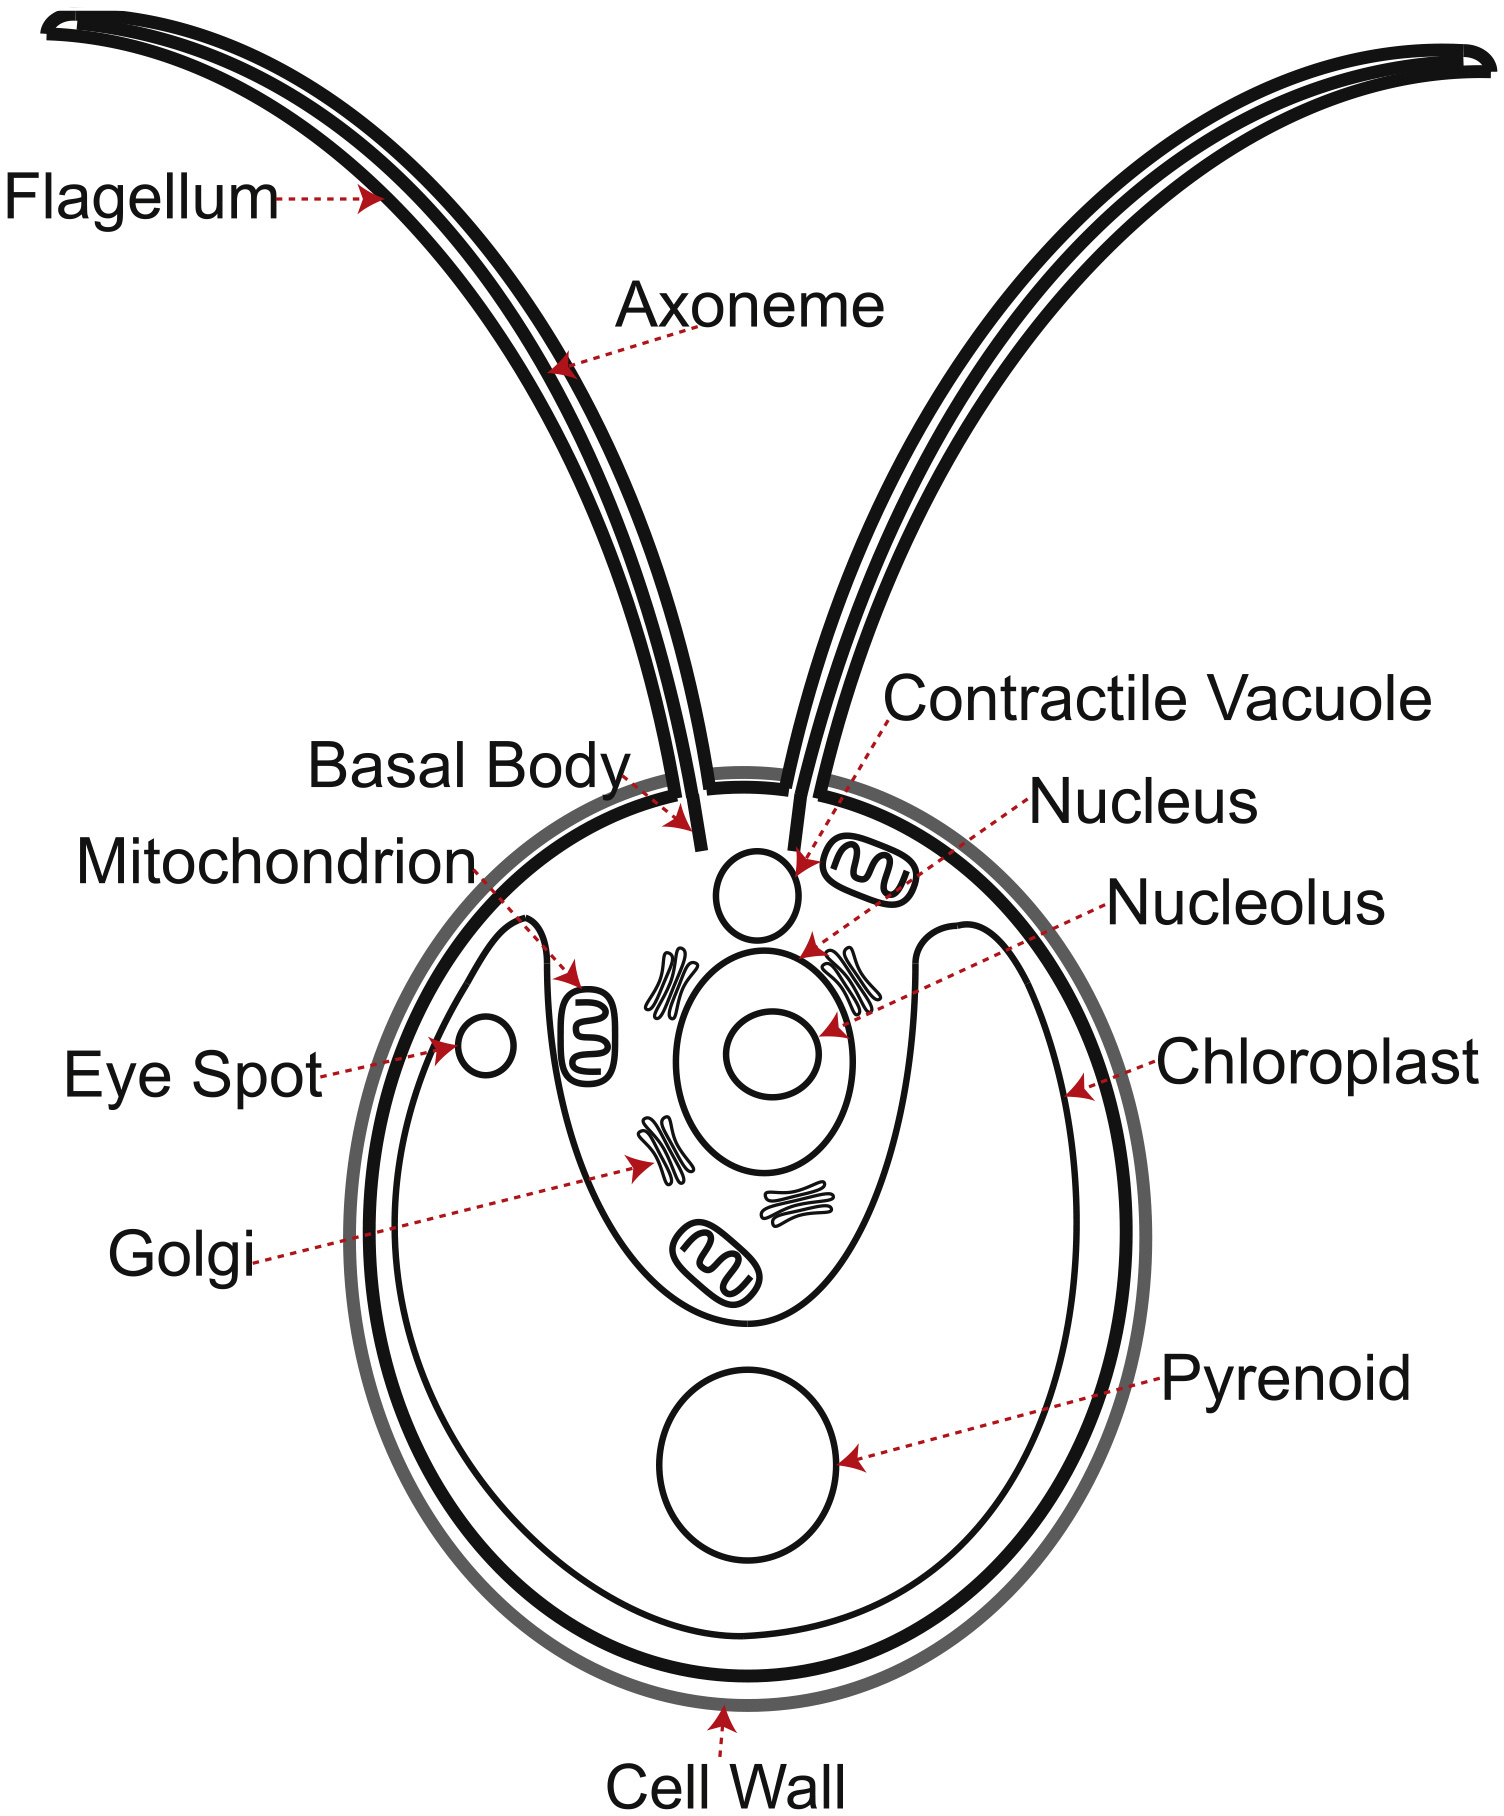
\includegraphics[width=\textwidth-80mm]{fig2-1.jpg}
%生成中英双语标题
{\setstretch{1.667}
\bicaption[fig:2.1]{图}{衣藻细胞结构示意图\ \citep{Avasthi2014}。图中标记的是已经鉴定的常见细胞器。}{Figure}{Diagram of the cell structure of a \textit{Chlamydomonas\/} cell \citep{Avasthi2014}. Prominent organelles identified are marked.}
\par}
%结束图片浮动体环境
\end{figure}

\subsection{衣藻作为模式生物的优势}
作为研究光合作用、油脂代谢、趋光性\ \citep{Kianianmomeni2014}、鞭毛的形成与解聚、鞭毛运动、蛋白质合成、细胞壁合成、配子形成、细胞周期调控和交配等过程的模式生
物\ \citep{Mussgnug2015,Gallaher2015,Flowers2015},衣藻具有以下特征和优势:

\begin{asparaitem}[\DiamondSolid]
\item 生长迅速,倍增时间仅\ 8-12\ 小时\citep{Blaby2014}。

\item 培养简便,成本低\ \citep{Sager1953,Harris1989,Flowers2015}。 此外,衣藻的细胞周期可以简单的通过调节光暗比进行同步\ \citep{Blaby2014,Hlavova2016}。

\item 在光照条件下,衣藻可进行光能自养。在黑暗条件下,衣藻可在含醋酸根离子的培养基中通过化能异养生存\ \citep{Blaby2014,Flowers2015}。这种灵活的代谢特性使得研究人员可以筛选出无法进行光合作用的突变体进而对光合作用相关基因进行研究\ \citep{Jinkerson2015}。

\item 衣藻鞭毛与哺乳动物细胞上的鞭毛高度同源,这使得衣藻可以作为研究纤毛相关疾病的模式系统。而且衣藻鞭毛是非必须的,这使得研究人员可以筛选出鞭毛结构和功能缺陷的突变体从而开展相关
    研究\ \citep{Blaby2014}。

\item 因衣藻既可进行有性繁殖,又可进行无性繁殖,所以可对其进行经典遗传学
    分析\ \citep{Kates1964,Flowers2015} (图\ \ref{fig:2.2})。 衣藻的营养细胞是单倍体。在缺氮条件下,营养细胞可以形成单倍体配子\ \citep{Gallaher2015}。 两种不同交配型的配子(mt+\ 和\ mt-)可以结合形成二倍体合子(图\ \ref{fig:2.2})。合子细胞没有鞭毛,它是这种生物在泥土中的休眠形式。在光照条件下,合子细胞可进行减数分裂产生四个有鞭毛的营养细胞。但是在生长条件良好的情况下,减数分裂产生的四个子细胞在从母细胞壁中释放之前会进行二到三轮有丝分裂。这样母细胞壁中就可能出现四、八或十六,甚至更多子细胞\ \citep{Jinkerson2015}。

\item 衣藻在营养生长阶段为单倍体,便于筛选突变体\ \citep{Avasthi2013,Li2016}。 突变后可立刻观察到表型而不需要进行杂交\ \citep{Jinkerson2015,Mussgnug2015}。

\item 针对衣藻的转化技术已经非常成熟。利用基因枪、玻璃珠转化或者电转化可以将外源\ DNA\ 导入到核基因组中\
    \citep{Jinkerson2015,Mussgnug2015,Kang2015,Neupert2009,Yamano2013}。 虽然是随机插入,但是插入位点的侧翼序列可以通过巢式\ PCR\ 和二代测序进行鉴定\
    \citep{Gonzalez-Ballester2011,Primers2007,Zhang2014,Li2016,Cheng2017}。尽管效率较低,外源\ DNA\ 也可通过同源重组定向插入到叶绿体和线粒体基因组中\ \citep{Kindle1990,Shimogawara1998}。 此外,衣藻中可用的筛选标记也非常丰富,如巴龙霉素抗性基因、潮霉素抗性基因、壮观霉素抗性基因、锌霉素抗性基因、卡那霉素抗性基因和四环素抗性基
    因等\ \citep{Mussgnug2015,Garcia-Echauri2015,Cerutti1997,Barahimipour2016}。 报告基因如氧气依赖的荧光蛋白\
\citep{Shaner2013,Harris2016,Ormo1996,Fuhrmann1999,Franklin2002,Hakkila2003,Heim1995,Phillips2001,Prasher1992,Onishi2016,Rasala2014,Lauersen2015}
    、黄素依赖的荧光蛋白\ \citep{Mukherjee2015}、 荧光素酶\
    \citep{Minko1999,Shao2008,Fuhrmann2004,Lauersen2013}、木聚糖酶\ \citep{Rasala2012}、 芳基硫酸酯酶\ ARS2\ \citep{Specht2014} 及各种细胞器靶向标记物也已被广泛使
    用\ \citep{Minko1999,Lauersen2015,Rasala2014}。

%开始图片浮动体环境,其中!表示取消严谨限制,h表示在此处插入,t表示在本页或下一页顶部插入
\begin{figure}[tbhp]
%居中对齐
\centering
%设置图片搜索路径,每个路径用{}括起来
\graphicspath{{figures/}}
%插入图片并设置图片宽度为文本宽度减10mm
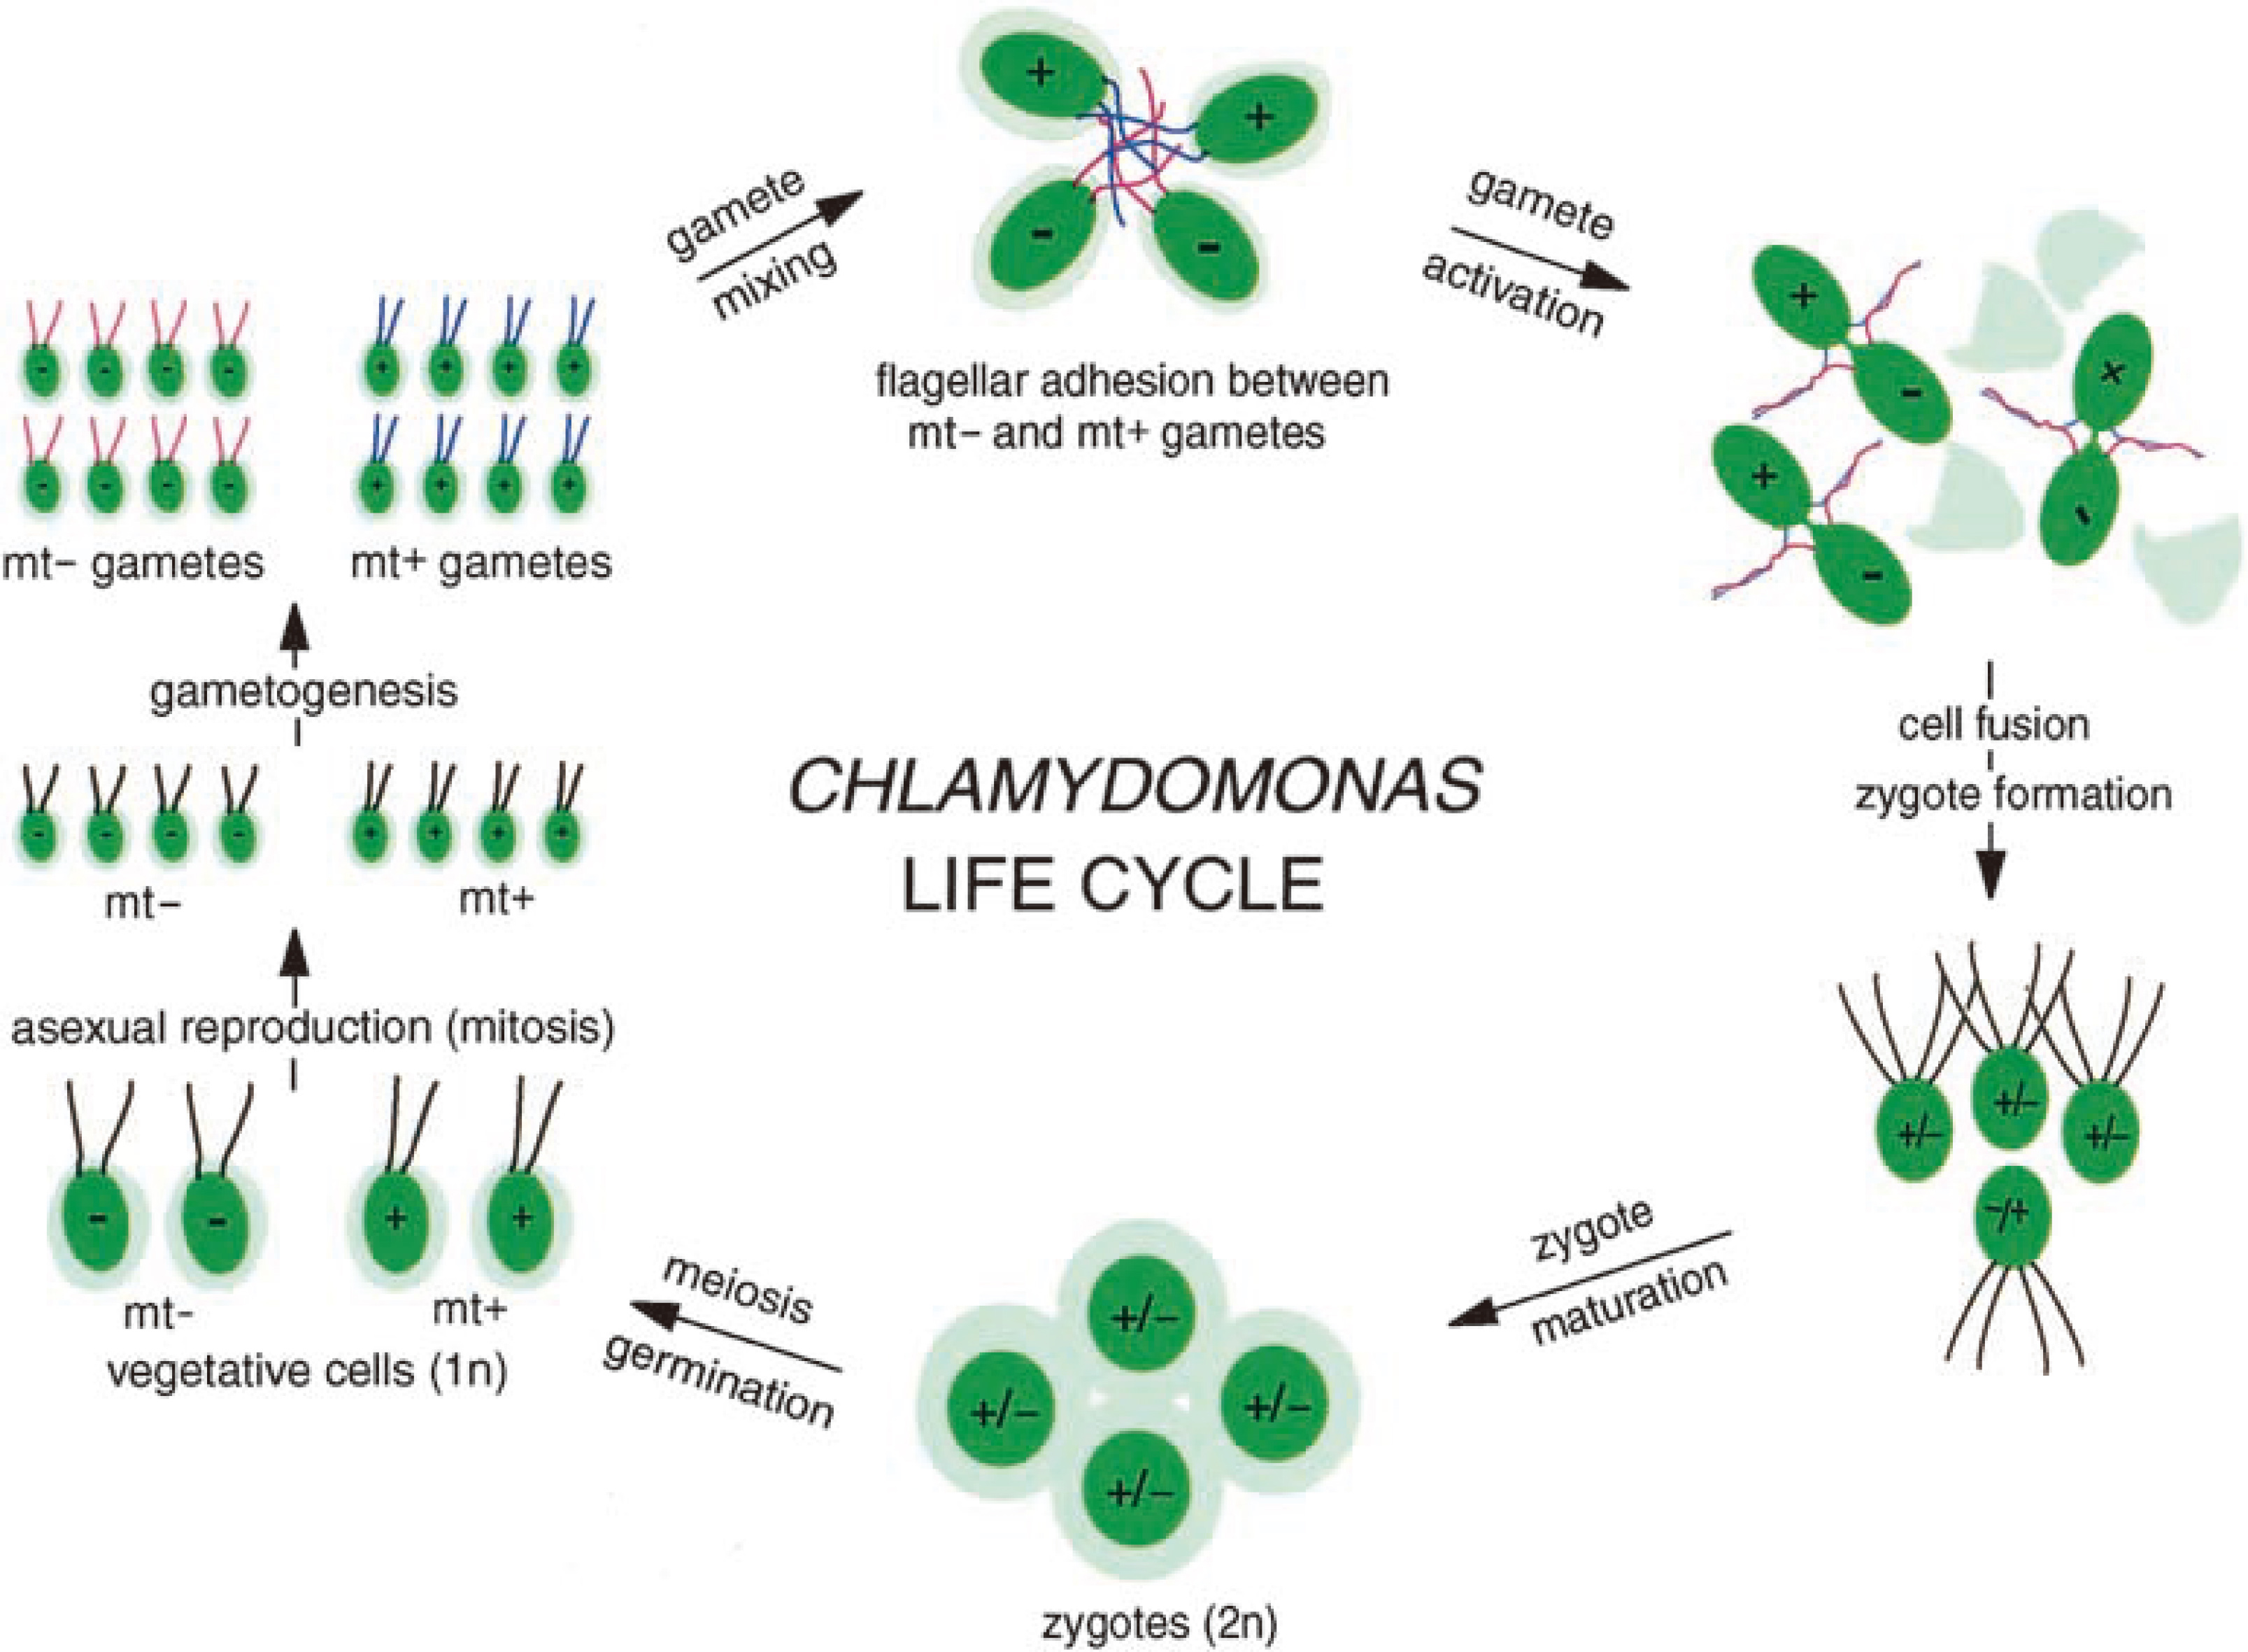
\includegraphics[width=\textwidth-10mm]{fig2-2.jpg}
%生成中英双语标题
{\setstretch{1.667}
\bicaption[fig:2.2]{图}{衣藻生活史示意图\ \citep{Zhao2001}。图中加号(+)代表正配子,减号(-)代表负配子。}{Figure}{Diagram of the \textit{Chlamydomonas reinhardtii}'s life cycle \citep{Zhao2001}. Plus sign and minus sign represent mating type plus and minus respectively.}
\par}
%结束图片浮动体环境
\end{figure}

\item RNA干扰已被广泛用于衣藻核基因的敲降\
    \citep{Hu2014,Schmollinger2010,Zhao2009,Molnar2009}。Cre/loxP\ 系统也已开始在衣藻中
    应用\ \citep{Kasai2016}。 尽管效率有待提高,锌指核酶和\ TALEs\ 已被用于衣藻核基因的编辑\
    \citep{Jinkerson2015,Mussgnug2015}。 近年来被广泛应用的基因魔剪\ CRISPR/Cas9\
    也已被用于衣藻研究,但这种方法在衣藻中的应用需要进一步开发\
    \citep{Jiang2014,Shin2016,Baek2016,Lander2016a}。

\item 关于衣藻的遗传信息非常丰富
\footnote{\textit{Chlamydomonas} Resource Center, www.chlamycollection.org},其核基因组、线粒体基因组和叶绿体基因组均以被测定\
    \citep{Grossman2003,Maul2002,Mussgnug2015,Gallaher2015,Flowers2015}。衣藻核基因组含十七条染色体\
    \citep{Dutcher1991},约\ 111.1\ Mbp,含\ 17741\ 个基因,叶绿体基因组约\ 203 kbp,含\ 99\ 个基因,线粒体基因组约\ 16 kbp,含\ 8\ 个基因\ \citep{Jinkerson2015,Mussgnug2015}。此外还有大量的\ EST\ 信息可供查询
    \footnote{\textit{Chlamydomonas reinhardtii} EST index, http://est.kazusa.or.jp/en/plant/chlamy/EST/}。 有可供使用的柯斯质粒和酵母人工染色体文库及\ BAC\ 文库\
    \citep{Blaby2014}。

\item 衣藻存在碳浓缩机制,对相关基因的研究和利用有望增强\ C3\ 植物的光合作用效率\
    \citep{Wang2011,Wang2014b,Atkinson2015,Grossman2007}。 此外,衣藻在缺氮条件下可以积累达细胞干重\ 20-30\%\ 的三酰甘油,可用于制备生物柴油\ \citep{Ho2014}。衣藻在缺硫条件下可积累氢气,是生产这种清洁能源的理想生物反应器\ \citep{Ho2014}。

\end{asparaitem}

鉴于这些优势,利用衣藻作为模式生物进行的研究逐年增多。除了传统的基础研究,衣藻在生物能源、生物医药等新技术领域的研究和应用也逐渐成为热点\
\citep{Franklin2004,Fuhrmann2004,Leon-Banares2004,Mayfield2007,Gallaher2015,Kempinski2015,Wijffels2010,Lauersen2013} 。在分子农业领域,经过遗传改造的衣藻已被用于生产哺乳动物血清淀粉蛋白、人抗体蛋白、人血管内皮生长因子、人乳头瘤病毒疫苗、HIV\ 抗原\ P24\ 等生物制剂\ \citep{Barahimipour2016}。 同时,衣藻在产氢和产油等方面的研究也正在如火如荼的开
展\ \citep{Gallaher2015,Flowers2015,Kempinski2015,Greenly2015}。

%开始图片浮动体环境,其中!表示取消严谨限制,h表示在此处插入,t表示在本页或下一页顶部插入
\begin{figure}[htb!]
%居中对齐
\centering
%设置图片搜索路径,每个路径用{}括起来
\graphicspath{{figures/}}
%插入图片并设置图片宽度为文本宽度减10mm
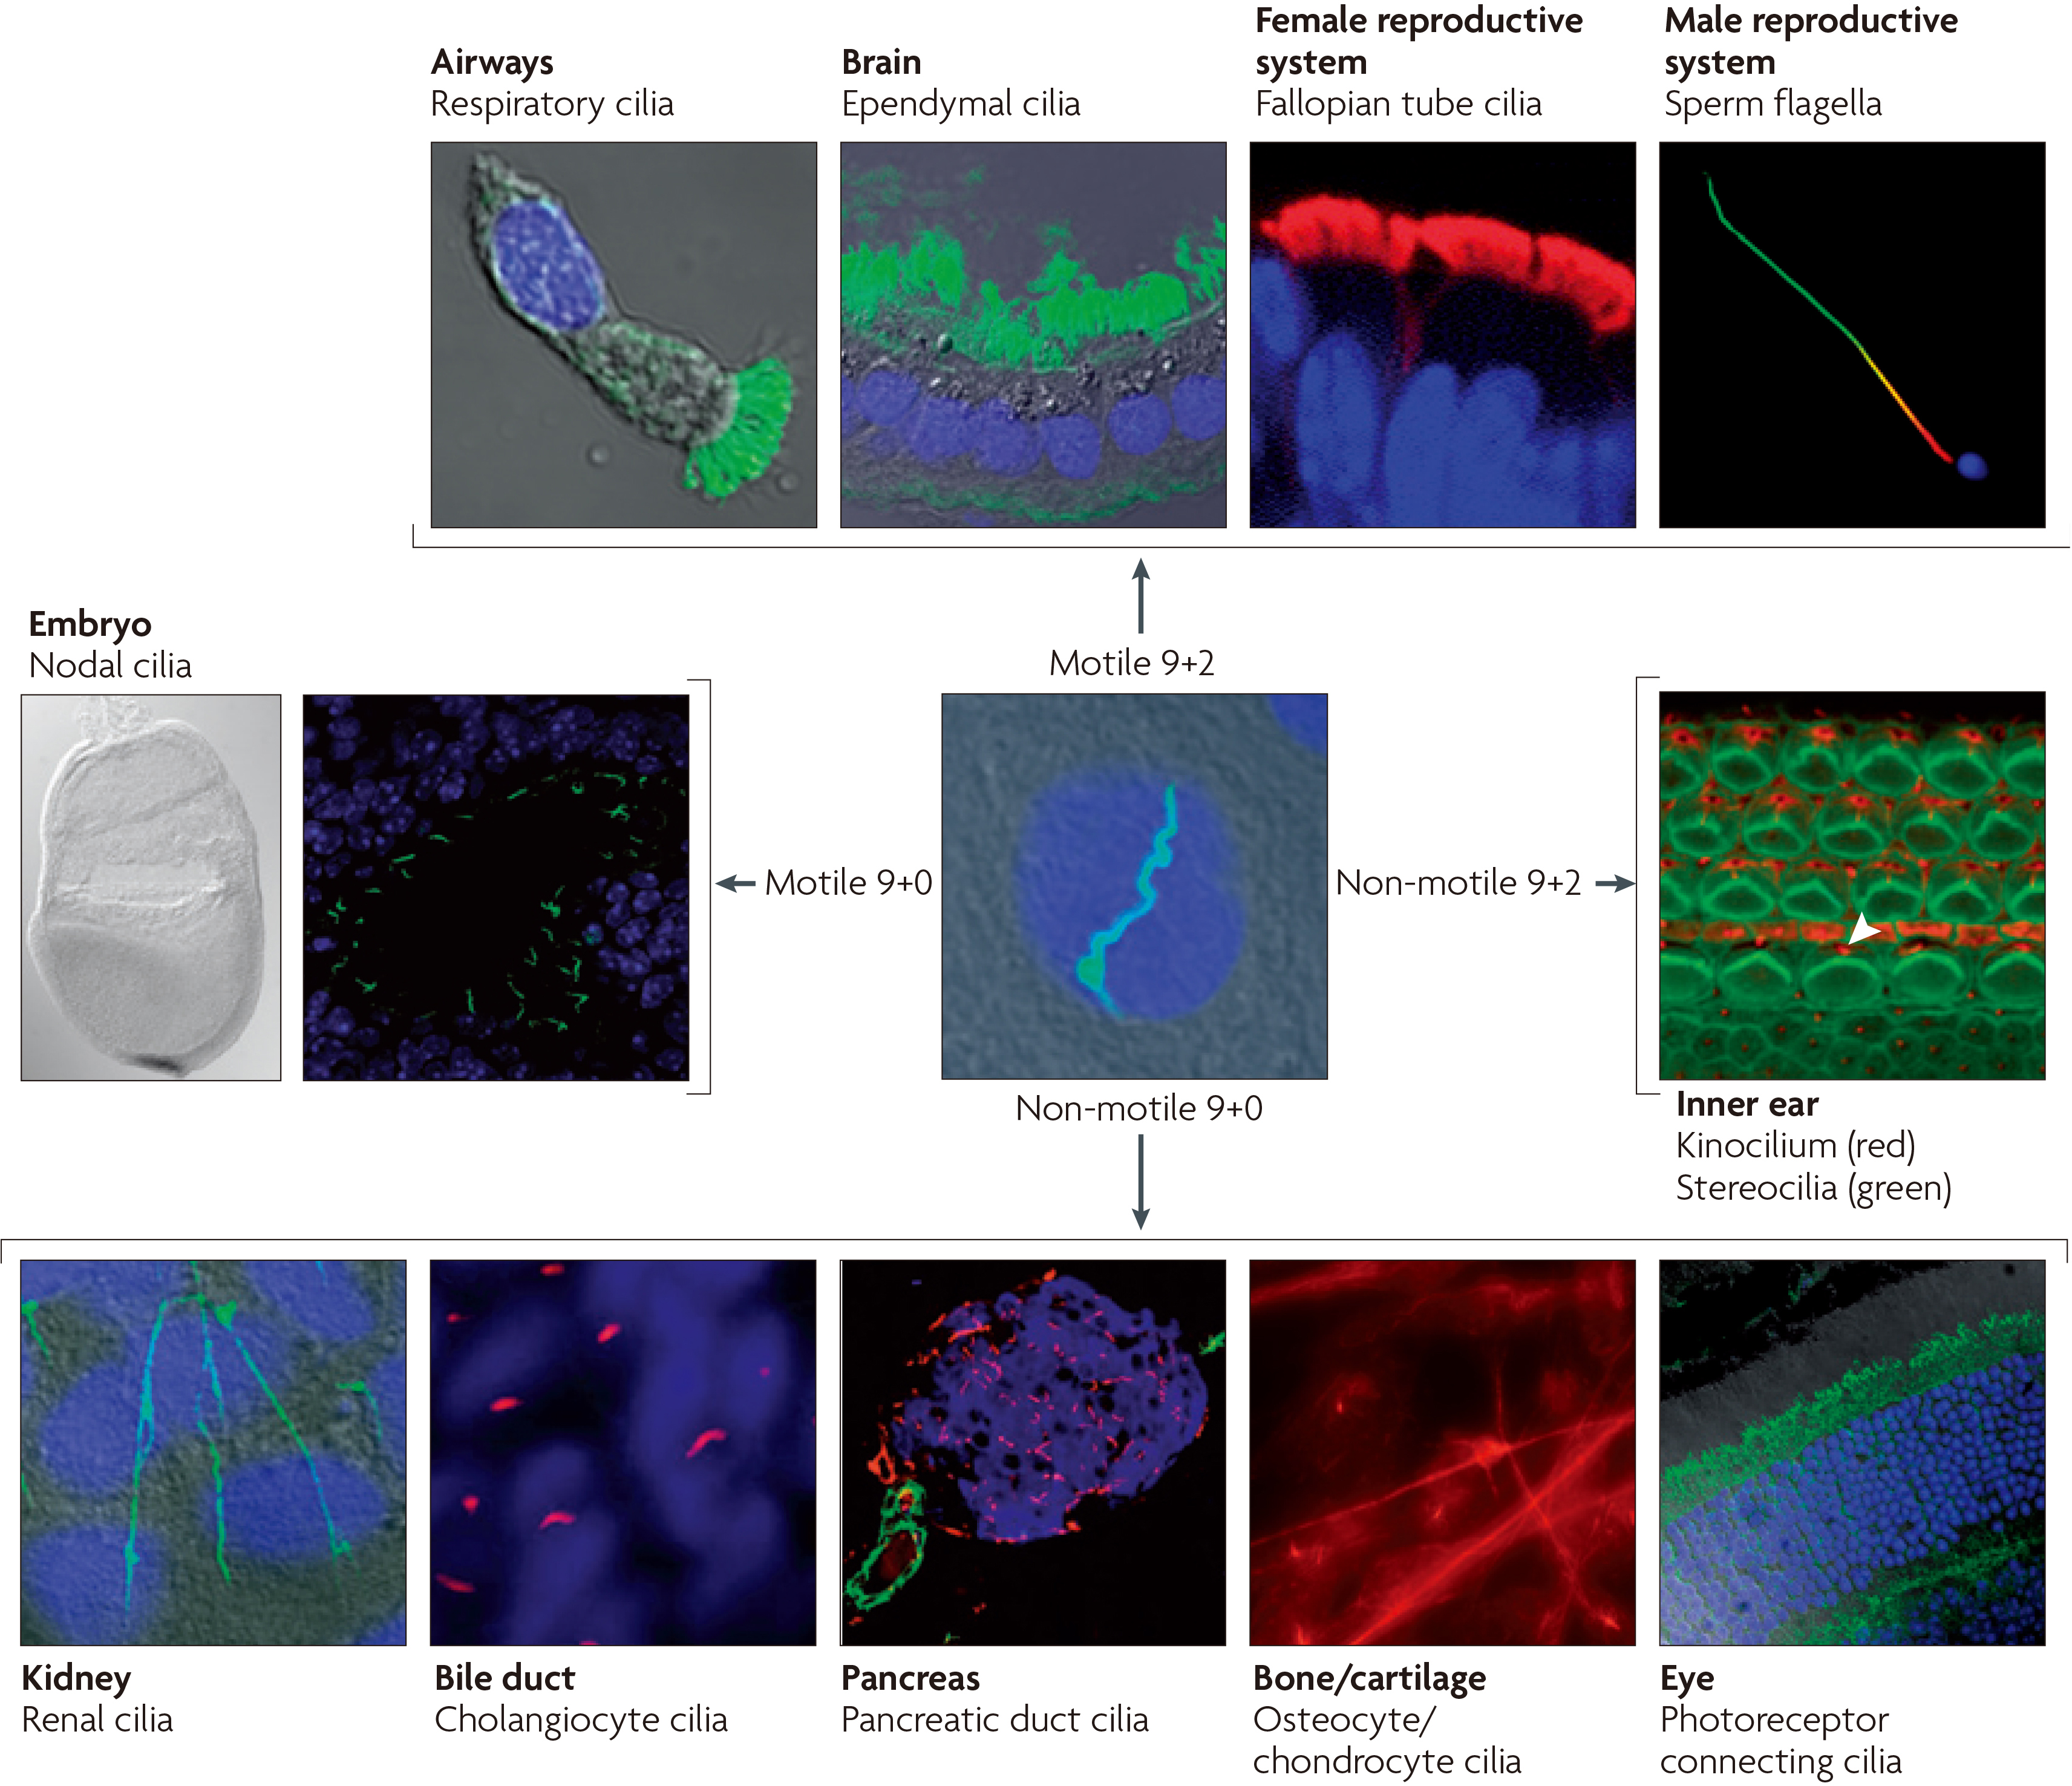
\includegraphics[width=\textwidth]{fig2-5.jpg}
%生成中英双语标题
{\setstretch{1.667}
\bicaption[fig:2.5]{图}{人体各种类型的细胞表面均有纤毛分布\ \citep{Fliegauf2007}。}{Figure}{Cilia extend from the surface of almost all cell types of the human body \citep{Fliegauf2007}.}
\par}
%结束图片浮动体环境
\end{figure}

\section{鞭毛简介}
\subsection{鞭毛的结构}
鞭毛从十九世纪末期被发现至今已有一百多年的历史,它们是一类保守的细胞器(图\ \ref{fig:2.5})。除酵母和高等植物外,鞭毛存在于几乎所有真核细胞
表面\ \citep{Czarnecki2012,Wheatley1996,Brooks2014,Fliegauf2007}。 鞭毛的形态和结构具有多样性,但总体上可被分为运动纤毛(出现在少数类型细胞上,一般为多生)和初级纤毛(出现在多种类型细胞上,一般为单生)两大类\ \citep{Gluenz2010,Gibbons1960}(图\ \ref{fig:2.5})。运动纤毛为\ 9+2\ 结构,初级纤毛为\ 9+0\ 结构。需要注意的是节点纤毛\footnote{nodal cilia}虽然为\ 9+0\ 结构,但可以借助\ A\ 管上的动力臂进行
运动\ \citep{Czarnecki2012} (图\ \ref{fig:2.5})。 在这两类纤毛中,运动纤毛一般出现在多纤毛细胞上且在进化上可能早于初级纤毛\ \citep{Warner2013}。鞭毛结构的这种保守性使得其直径维持在\ 160-280 nm \ 之间\
\citep{Huang2016}。其中纤毛基部偏粗,远端偏细\ \citep{Huang2016}。 这一方面是因为基部存在突起(可能是将要分泌到环境中的囊泡),另一方面是因为微管二联管在远端变成单管\
\citep{Huang2016,Wang2014,Wood2013}。

基于鞭毛结构的保守性,这里我们主要介绍衣藻鞭毛的结构。正常的衣藻细胞有两根运动鞭毛,靠近眼点的称为顺式鞭毛\footnote{cis flagellum},远离眼点的称为反式鞭毛\footnote{trans flagellum}。衣藻鞭毛主要由轴丝、过渡区、鞭毛颈(纤毛膜外部的蛋白鞘)和鞭毛膜
以基体为模板形成\ \citep{Hilbert2016,Kitagawa2011}。基体为特化的中心粒(图\ \ref{fig:2.6})。轴丝为\ 9+2\ 结构,外部九个二联管的\ A\ 管上伸出外部动力臂
\footnote{ODA, outer dynein arm}、内部动力臂\footnote{IDA, inner dynein arm}和放射辐条等结构
(图\ \ref{fig:2.6})。相邻二联管的\ A\ 管和\ B\ 管之间由连接蛋白连接\ \citep{Song2015}。ODA\ 和\ IDA\ 与相邻二联管的\ B
管相互作用,放射辐条则与环绕中央管的结构相互作用。从精细结构上来说,A\ 管和中央管都由十三根原纤维组成,B\ 管则仅含十根原纤维。

ODA\ 为鞭毛的摆动提供动力,而\ IDA\ 则是鞭毛产生正常的波形所必须的。前者结构简单,由三个动力蛋白重链
\footnote{DHC, dynein heavy chain;HC$\upalpha$、HC$\upbeta$\ 和\ HC$\upgamma$}和两个中间链
\footnote{IC, intermediate chain;IC78\ 和\ IC70}及至少十个轻链\footnote{LC, light chain}形成三头状复合物\ \citep{Fowkes1998}。IC\ 和\ HC\ 之间存在相互作用,IC\ 是维持\ HC\ 稳定所必须的。该复合物的一端与锚定复合物\footnote{DC, docking complex}结合,DC\ 含三个亚基,分别为\ DC25、DC63\ 和\ DC105\ \citep{Fowkes1998}。这种复合物在\ A\ 管上每隔\ \SI{24}{\nm}\ 出现一次\ \citep{Fowkes1998}。IDA\ 的结构则相对比较复杂。目前已鉴定到的\ IDA\ 复合物可被归为三类亚型:I1、I2\ 和\ I3。I1\ 和\ I2\ 均为单头状结构。I3\ 则为双头状结构,它由两个\ DHCs、 三个\ ICs\ 和三个\ LCs\ 组成。IDA\ 在\ A\ 管上出现的周期是\ \SI{96}{\nm}\ \citep{Oda2014},三种亚型复合物分别占据不同的位置\
\citep{Perrone1998}。 轴丝的中心区域是由中央鞘包裹的两根中央管,它与外部二联管之间的连接由放射辐条实现。

%开始图片浮动体环境,其中!表示取消严谨限制,h表示在此处插入,t表示在本页或下一页顶部插入
\begin{figure}[htb!]
%居中对齐
\centering
%设置图片搜索路径,每个路径用{}括起来
\graphicspath{{figures/}}
%插入图片并设置图片宽度为文本宽度减10mm
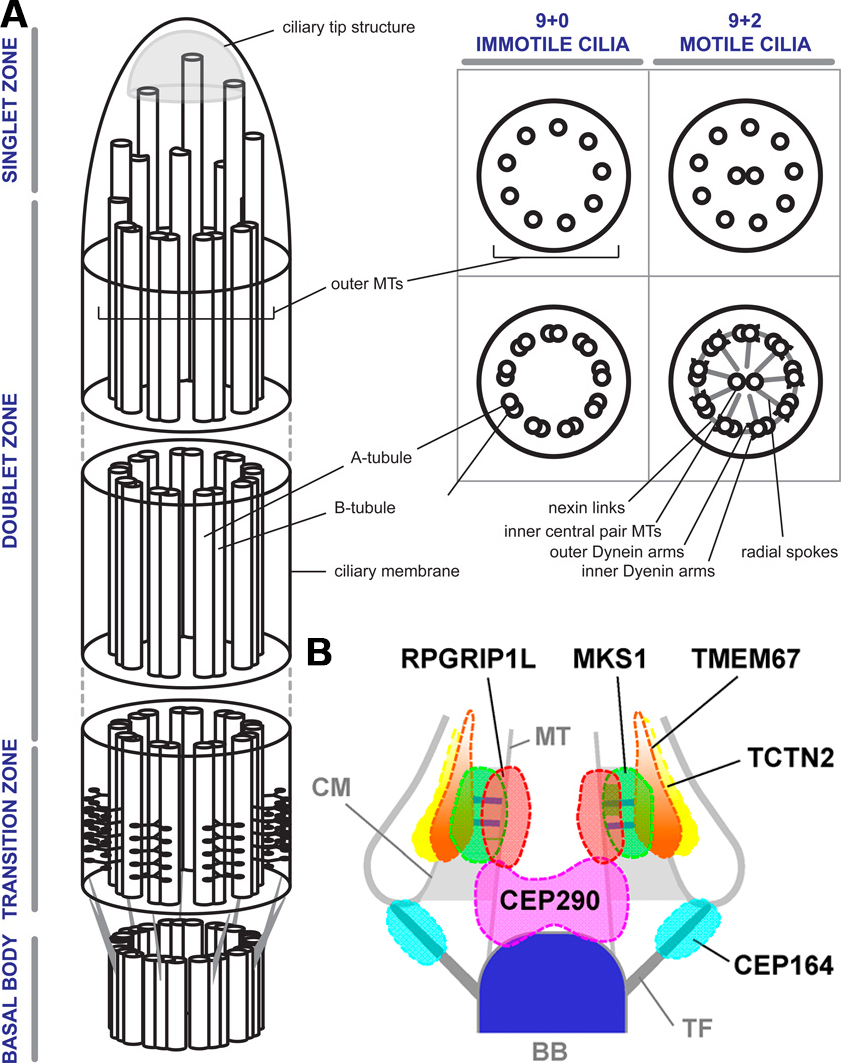
\includegraphics[width=\textwidth-10mm]{fig2-6.jpg}
%生成中英双语标题
{\setstretch{1.667}
\bicaption[fig:2.6]{图}{鞭毛结构模式图。(A)鞭毛轴丝和\ Y\ 形连接器模式图\ \citep{Czarnecki2012}。 (B)部分已知过渡区蛋白的相对位置\ \citep{Yang2015a}。}{Figure}{Schematic representation of ciliary structure. (A) Schematic representation of axonemes and Y-shape linkers \citep{Czarnecki2012}. (B) A localization model of part transition zone proteins at the ciliary base \citep{Yang2015a}.}
\par}
%结束图片浮动体环境
\end{figure}

过渡区指的是纤毛基体和轴丝之间的结构\ \citep{Czarnecki2012}。它由两部分组成:一是在三联管和二联管交界处从\ B\ 管上突出的过渡纤维,它们形成间隔\ \SI{60}{\nm}\ 左右的类似螺旋桨的结构(图\ \ref{fig:2.6})。二是外部二联管和纤毛膜之间的\ Y\ 形连接器\ \citep{Czarnecki2012}。其中后者有多层,它们是过渡区的主体(图\ \ref{fig:2.6})。在初级纤毛中,含\ Y\ 形连接器的区域对应的纤毛膜上有整齐排列的突起颗粒,该区域也被称为纤毛颈\ \citep{Czarnecki2012}。实际上,衣藻鞭毛的过渡区还包括二联管中央空腔中的桶形结构、连接\ A\ 管的星形纤维及纤毛膜和二联管之间的楔形结构\ \citep{Czarnecki2012}。

纤毛独特的生化组成表明存在特定的隔离机制对进入纤毛的跨膜和可溶性因子进行控制\ \citep{Ye2013}。越来越多的证据表明在纤毛过渡区中存在扩散屏障。在初级纤毛的纤毛膜和质膜间的扩散屏障包含胞裂蛋白\footnote{septin}\ \citep{Hu2010} 和\ B9\ 复合物\ \citep{Chih2011}。而过渡区中可溶性蛋白的扩散屏障可能有着与核孔类似的结构\
\citep{Kee2012,Huang2010}。然而,\citet{Breslow2013}\ 的结果表明这种扩散屏障既不同于神经元轴突起始端的肌动蛋白微丝屏障,也不同于核孔。

鞭毛膜的外表面覆盖着由富含羟脯氨酸的糖蛋白组成的糖萼\footnote{glycocalyx}\ \citep{Pigino2009}。糖萼的功能之一是参与有性生殖过程\ \citep{Cooper1983}。鞭毛膜的脂成分与质膜的组成有显著差异,前者富含胆固醇和鞘磷脂。它们是形成脂伐的主要成分\ \citep{Garcia-Gonzalo2015,Chavez2015}。最新的研究表明,在\ Inpp5e\
的作用下,纤毛膜富含\ PI(4)P,但其近端却富含\ PI(4, 5)P2\ \citep{Garcia-Gonzalo2015}。这种特殊的膜脂分布可影响纤毛膜蛋白\ Gpr161\
的定位进而调控\ Hh\ 信号通路\ \citep{Garcia-Gonzalo2015,Chavez2015}。 纤毛膜具有不对称性,膜上的信号分子一般聚集形成独特的微结构域\ \citep{Nechipurenko2013}。

\subsection{鞭毛的形成}

%开始图片浮动体环境,其中!表示取消严谨限制,h表示在此处插入,t表示在本页或下一页顶部插入
\begin{figure}[htb!]
%居中对齐
\centering
%设置图片搜索路径,每个路径用{}括起来
\graphicspath{{figures/}}
%插入图片并设置图片宽度为文本宽度减10mm
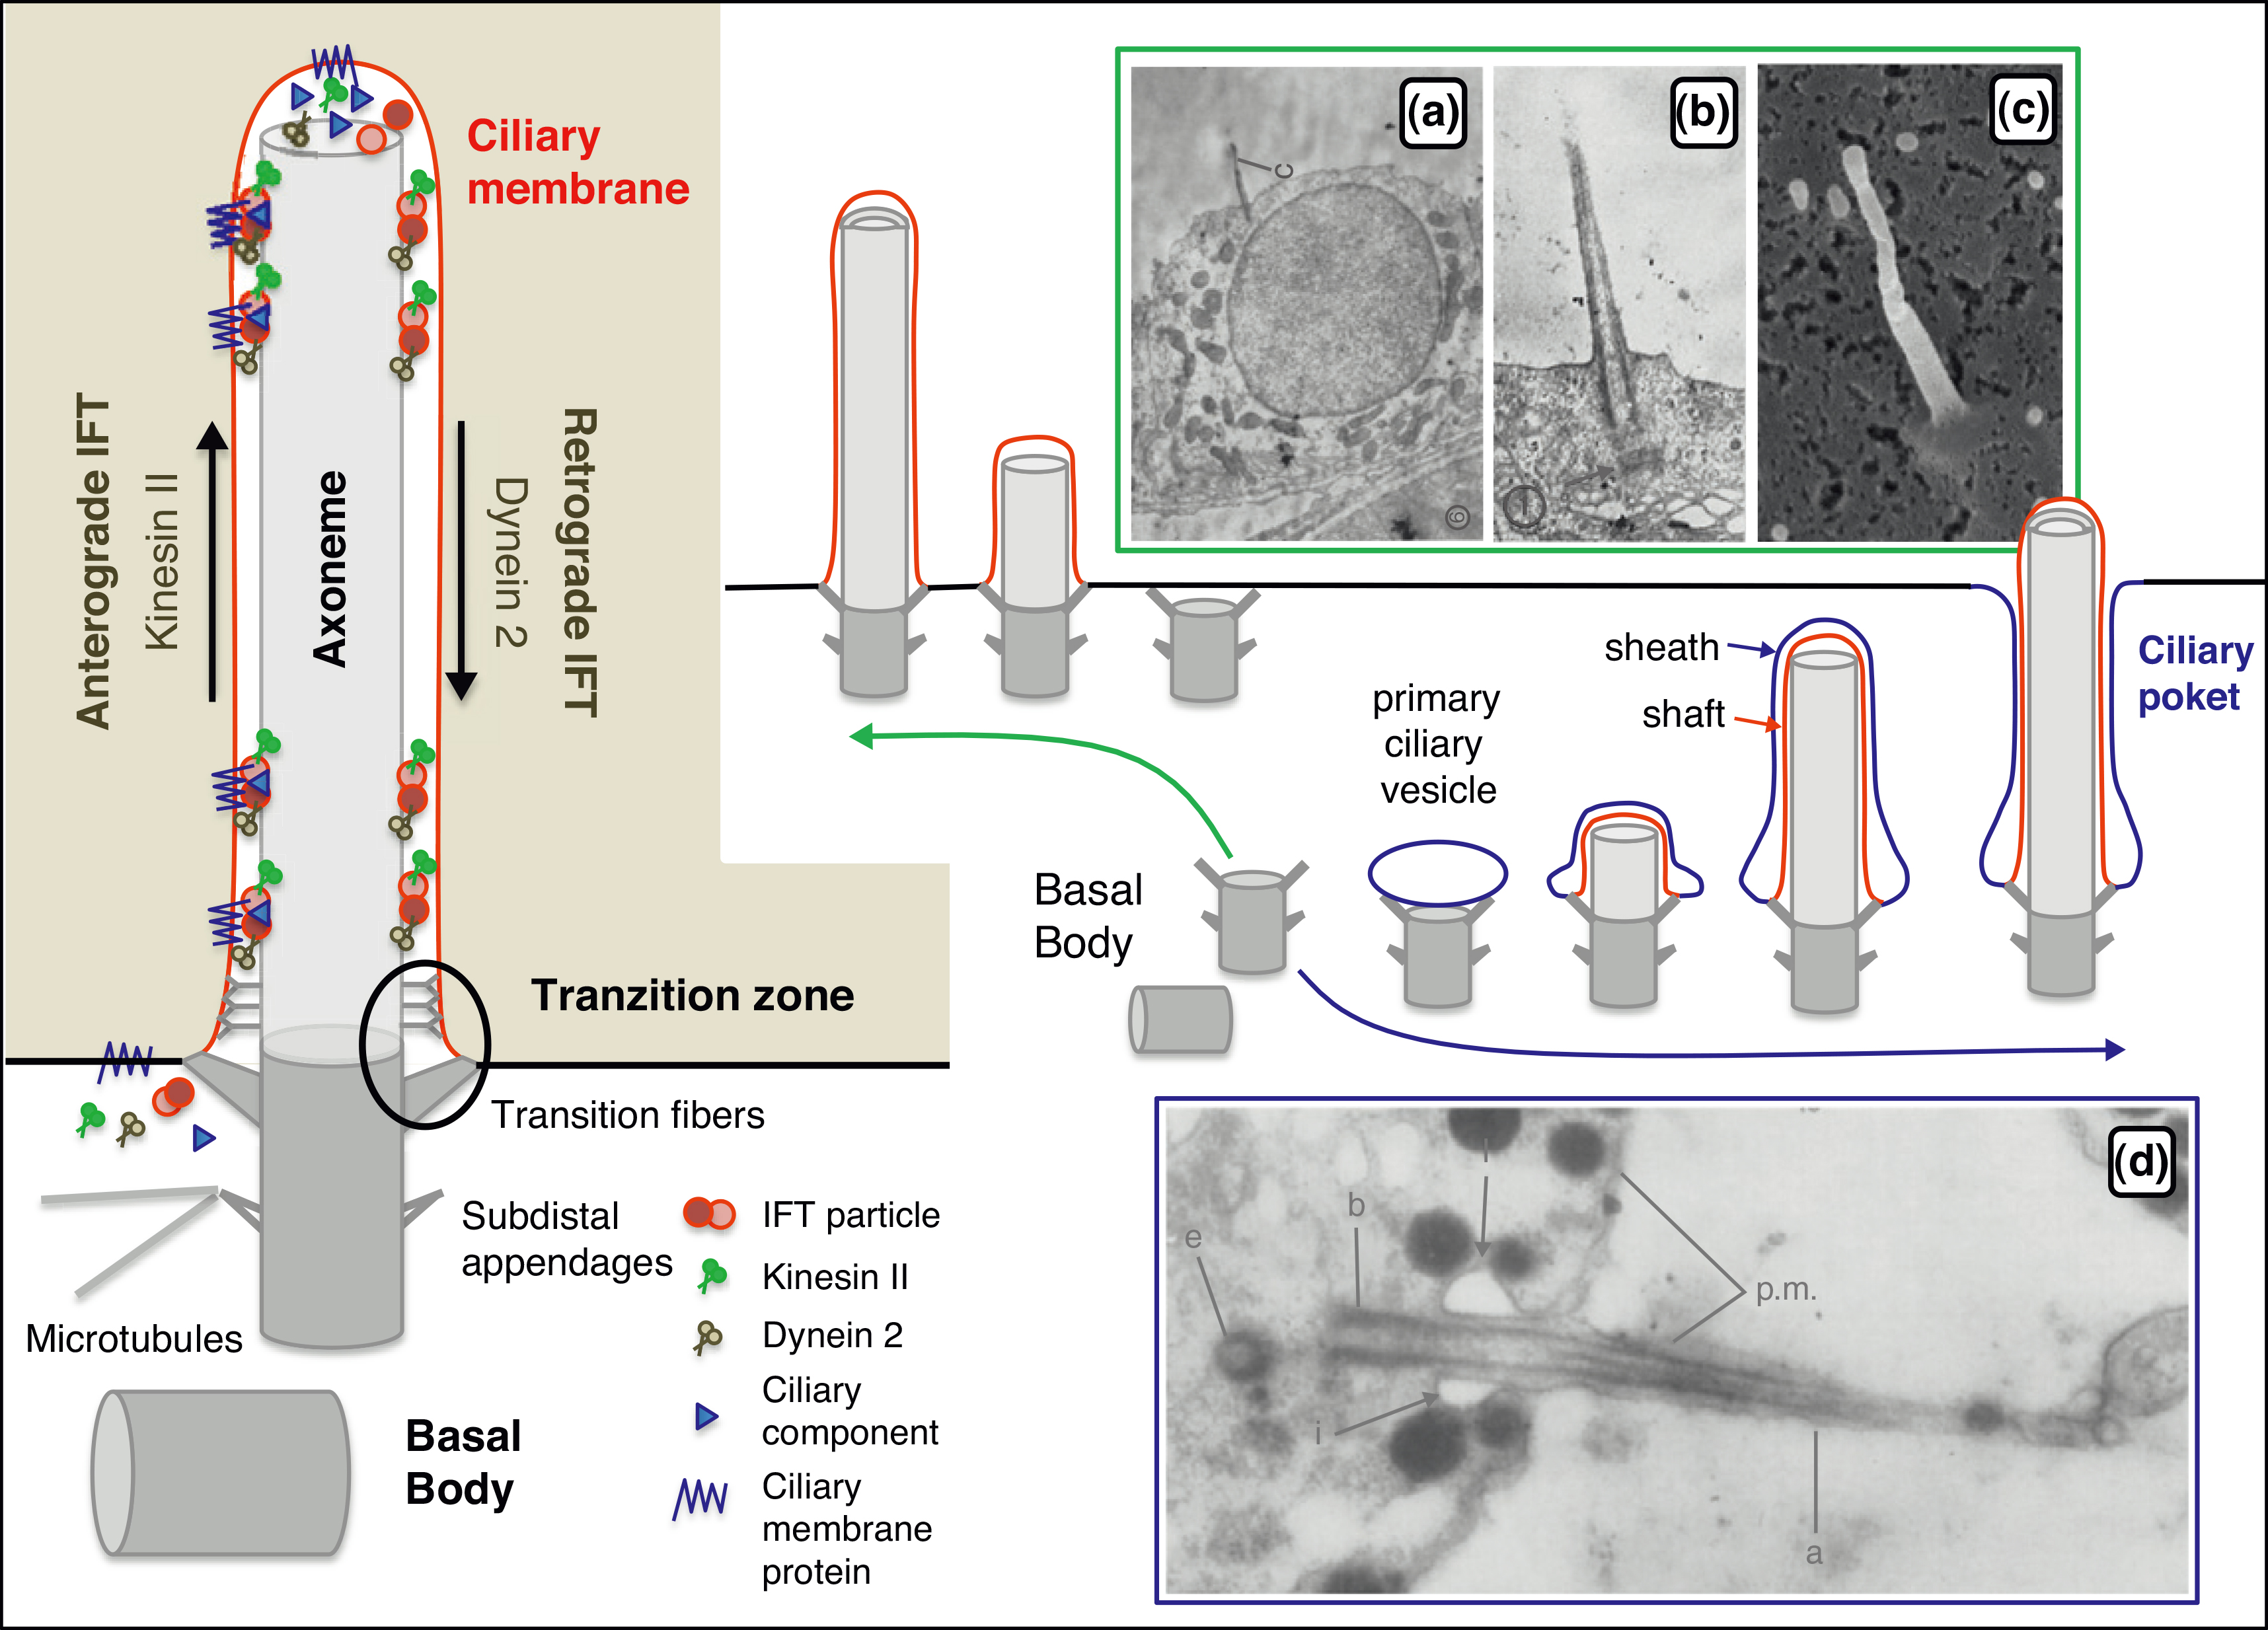
\includegraphics[width=\textwidth-20mm]{fig2-7.jpg}
%生成中英双语标题
{\setstretch{1.667}
\bicaption[fig:2.7]{图}{两种不同的初级纤毛形成途径\ \citep{Benmerah2013}。左侧显示的是纤毛和\ IFT\ 的模式图,右侧显示的是初级纤毛形成的胞内途径和胞外途径。a\ 和\ b\ 为通过胞外途径形成的初级纤毛的透射电镜照片,c\ 为通过胞外途径形成的初级纤毛的扫描电镜照片。d\ 为通过胞内途径形成的初级纤毛的透射电镜照片。}{Figure}{Two different primary ciliogenesis pathways  \citep{Benmerah2013}. Left, scheme showing the organization of the primary cilium (PC) and the IFT. Right, description of the two primary ciliogenesis pathways. (a, b) TEM pictures showing longitudinal section of PC in kidney tubules epithelial cells. (c) Scanning EM picture showing a PC at the apical surface of IMCD3 kidney cells. (d) TEM picture showing a longitudinal section of a primary cilium in secretory cells of the mouse adenohypohysis.}
\par}
%结束图片浮动体环境
\end{figure}

纤毛的形成过程大体上可分为两类:胞内途径和胞外途径\ \citep{Sorokin1968}(图\ \ref{fig:2.7}, \ref{fig:2.8})。两种途径形成的纤毛并无本质上的差异,只是在形态上略有不同(图\ \ref{fig:2.7})。比如通过胞内途径形成的纤毛有纤毛袋\footnote{ciliary pocket}\citep{Benmerah2013}\ 且绝大部分埋藏在细胞内,而通过胞外途径形成的纤毛突出在细胞表面\ \citep{Mazo2016}。 然而,部分细胞天然能够形成两种类型的纤毛,另一些细胞在外因的诱导下纤毛形成途径可发生转变\ \citep{Mazo2016}。比如在\ RPE1\ 细胞中,敲除\ C-Nap1\ 和\ CEP128\  可使约\ 30\%\ 的细胞形成表面纤毛\ \citep{Mazo2016}。

在胞内途径中,来自高尔基体的囊泡首先被招募到母中心粒的远端,随后轴丝延伸并挤压囊泡使其顶层膜与质膜融合,纤毛得以突出在细胞表面\ \citep{Sorokin1962,Sorokin1968}(图\ \ref{fig:2.8})。研究表明,远端附属蛋白、Cby\ 及\ Rab11/Rabin8/Rab8、BBSome、EHD1/3\ 等蛋白参与了这一过程
\ \citep{Burke2014,Lu2015,Westlake2011,Nachury2007,Knodler2010,Zhang2012}(图\ \ref{fig:2.8})。 在中心粒向质膜下方迁移过程中,远端附属蛋白\ CEP164
招募\ Cby\
形成环状结构,Cby\ 进而与\ Rabin8\
相互作用并促进\ CEP164/Rabin8\ 复合物的形成,Rabin8\
可招募并激活\ Rab8\ 从而促进来自高尔基体的小囊泡在中心粒远端聚集并融合成大的纤毛囊泡
\ \citep{Burke2014,Schmidt2012}。 纤毛囊泡形成后,微管亲和性调控激酶\ MARK4、 中心粒蛋白\ ODF2
\ \citep{Kuhns2013}、Centrin2 \citep{Prosser2015}\ 和\ TTBK2(Tau tubulin kinase 2)\citep{Goetz2012}\ 可以移除轴丝延伸抑制复合物\ Kif24/CP110/Cep97\
\citep{Spektor2007,Tsang2008,Tsang2013,Kobayashi2011},这使得轴丝向纤毛囊泡中延伸。最新的研究表明,磷酸酶\ Inpp5e\ 和磷酸激酶\ PIPKI$\upgamma$\ 这对催化互逆反应的蛋白可以通过控制基体中\ PI(4)P\
的浓度影响\ TTBK2\ 的招募和\ CP110\
的移除\ \citep{Xu2016a}。这是纤毛形成起始过程中重要的控制机制,其他磷脂相关生化过程在纤毛形成中也可能发挥了重要作用\ \citep{Xu2016a}。

胞外途径相对而言比较简单且研究较少\ \citep{Benmerah2013}。具体而言,母中心粒通过过渡纤维直接锚定在质膜上,轴丝的延伸使得纤毛突出到胞外环境\ \citep{Benmerah2013}(图\ \ref{fig:2.7})。衣藻鞭毛的形成过程类似于胞外途径,不同之处在于其两个中心粒均能够作为基体形成鞭毛。

%开始图片浮动体环境,其中!表示取消严谨限制,h表示在此处插入,t表示在本页或下一页顶部插入
\begin{figure}[htb!]
%居中对齐
\centering
%设置图片搜索路径,每个路径用{}括起来
\graphicspath{{figures/}}
%插入图片并设置图片宽度为文本宽度减10mm
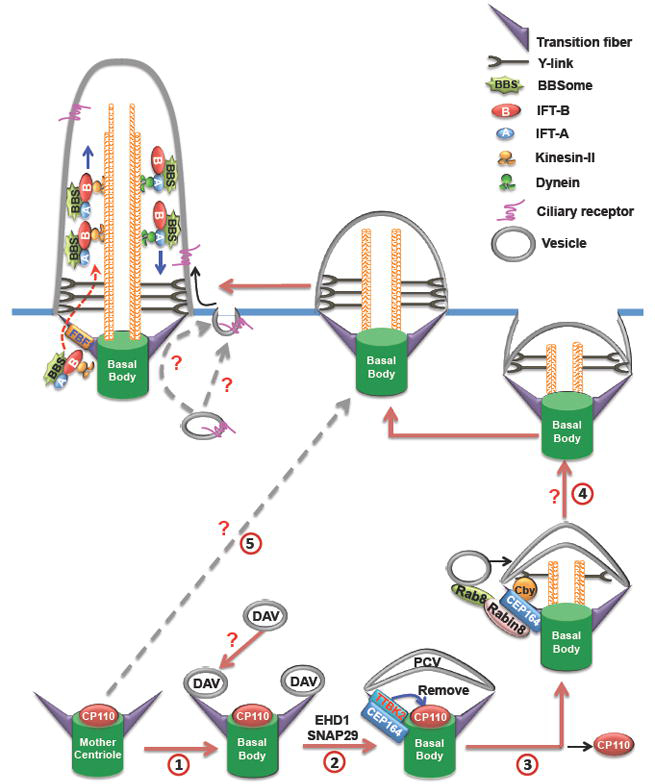
\includegraphics[width=\textwidth-20mm]{fig2-8.jpg}
%生成中英双语标题
{\setstretch{1.667}
\bicaption[fig:2.8]{图}{胞内途径初级纤毛形成过程示意图\ \citep{Wei2015}。TF\ 代表过渡纤维,TZ\ 代表过渡区,DA\ 代表远端附属物,DAV\ 代表远端附属囊泡,PCV\ 代表初级纤毛囊泡,问号代表未知途径。}{Figure}{Ciliogenesis of primary cilia through intracellular pathway \citep{Wei2015}. TFs, transition fibers; TZ, transition zone; DAs, distal appendages; DAVs, distal appendage vesicles; PCV, primary ciliary vesicle. Question mark represents unknown mechanism.}
\par}
%结束图片浮动体环境
\end{figure}

\subsection{鞭毛的解聚}
纤毛解聚发生在纤毛顶端,解聚时纤毛组分被回收到细胞体中\ \citep{Liang2016,Pan2005,Marshall2001}。 已知在三种情况下纤毛会发生解聚:环境压力、细胞分化和细胞增殖\ \citep{Liang2016}。对哺乳动物细胞上的初级纤毛而言,机械力和热激会导致纤毛解聚\ \citep{Liang2016}。对衣藻等原生动物而言,渗透压和某些化学物质会导致纤毛解聚,如氯化钠、ATP、GTP、焦磷酸钠和柠檬酸盐等\ \citep{Liang2016}。单细胞生物和哺乳动物细胞在细胞分化过程中均会发生纤毛解聚,但其具体功能尚未研究透彻。由于纤毛的基体是由中心粒转变而来,而中心粒在细胞增殖过程中需要形成纺锤体,故绝大多数纤毛在细胞增殖过程中会发生解聚从而释放中心粒。已知的例外有果蝇的精母细胞,其在减数分裂过程中依然保留纤毛\ \citep{Riparbelli2012}。已有研究表明,大多数细胞在\ G1,S\ 和\ G2\ 期均有纤毛,但在\ M\ 期纤毛消失\ \citep{Liang2016}。鞭毛解聚可能在细胞\ G1/S\ 转变过程中扮演重要角色\ \citep{Liang2016}。

纤毛是一种包含上千种蛋白的有复杂亚结构的细胞器\ \citep{Rohatgi2010},解聚过程中发生的一系列生化反应将它们运回细胞体,如微管的去乙酰化和解聚,蛋白磷酸化、甲基化和泛素化
等\ \citep{Liang2016,Meng2016a,Hu2015,Huang2009,Long2015}。一些保守的信号分子和信号通路参与了纤毛解聚过程,如钙离子、cAMP\ 和\ aurora\ 激酶等\ \citep{Liang2016,Hu2015,Meng2016a,Hu2015a}。此外,鞭毛可通过微泡将特定蛋白分泌到胞外\ \citep{Wood2015,Wang2016,Long2016}。研究表明鞭毛在解聚过程中微泡的分泌量增加\ \citep{Long2016}。 抑制鞭毛的微泡分泌可在一定程度上减缓鞭毛
解聚过程\ \citep{Long2016}。这些结果表明鞭毛解聚过程部分鞭毛膜脂和膜蛋白可能以微泡的形式分泌到胞外\ \citep{Long2016}。

\subsection{鞭毛的功能}
鞭毛是细胞的运动器官之一,同时它也作为细胞天线参与信号传导与释放\
\citep{Marshall2006,Singla2006}。

鞭毛的运动功能主要体现在三个方面:一是驱动细胞自身的运动。衣藻通过鞭毛进行的运动是其具有趋光性的原因之一\ \citep{Okita2005,Wakabayashi2011}。此外,鞭毛驱动的精子的运动是完成受精所必须
的\ \citep{Turner2003}。 二是通过周期性运动使细胞周围的液体发生移动。支气管内表皮细胞上的多纤毛通过运动可以清除痰液和细菌\
\citep{Marshall2006}。脊椎动物胚胎发育早期,胚结细胞表面的纤毛通过顺时针方向运动造成某些信号分子的极性分布从而决定体轴的方向\ \citep{Hirokawa2006}。此外,脑脊液的流动也依赖纤毛的运动。三是推动其他细胞发生移动。雌性输卵管表皮的纤毛通过运动促进卵子排出,这对完成受精是必须的。

鞭毛内富集了大量信号分子和受体,它们参与的信号传导,对机体的生存至关重要。如视觉、嗅觉、听觉及胚胎发育等\ \citep{Singla2006}。以视觉为例,视网膜的核心视杆- 视锥细胞的外节由异化的纤毛组成
(图1.4),
感光色素即位于其中\ \citep{Arden1979,Palczewski2006}。 Sonic Hedgehog
\ 和\ Wnt\
信号通路是调控动物发育的两条重要途径,它们都和纤毛有关\
\citep{Caspary2007,Dutta2015,Liu2014a}。 Hedgehog\ 信号通路的重要因子\ Ptch1\ 及\ Smo\ 在初级纤毛上起作用(图1.5),纤毛缺陷造成\ Hedgehog\ 信号传导途径不能正常进行,从而影响动物的发育\
\citep{Jiang2008,Liu2014a}。Inversin\ 是纤毛中调控动物内脏左右不对称的蛋白,研究表明它可能是经典和非经典\ Wnt\ 信号传导途径相互转换的开关。

此外,单细胞的衣藻到高等哺乳动物细胞的纤毛均能够释放和结合胞外囊泡\ \citep{Wood2015,Wang2016}。
胞外囊泡\footnote{extracellular vesicles} 可被分为两类:外泌体\footnote{exosome}和
微泡\footnote{ectosome}\ \citep{Cocucci2015,Gould2013}。前者由多囊泡体
\footnote{multivesicular body}通过胞吐释放到胞外,后者由细胞膜或特化的细胞膜如纤毛膜、鞭毛膜和膜纳米管通过出芽形成\ \citep{Cocucci2015,Gould2013}。胞外囊泡中含有脂类、蛋白和核酸,能够进行短距离和长距离通讯,同时介导一系列的生理和病理过程\ \citep{Raposo2013,E.L.Andaloussi2013}。

衣藻从纤毛顶端释放微泡,这些微泡中所含蛋白与交配及母细胞壁的降解有关\
\citep{Wood2013,Wang2016,Wood2015,Cao2015}。与纤毛膜相比,衣藻纤毛分泌的微泡富含蛋白酶、转运必需内体分选复合物蛋白\footnote{ESCRT, endosomal sorting complex required for transport}、小鸟苷三磷酸酶和泛素化蛋白\ \citep{Long2016}。布氏锥虫通过鞭毛分泌胞外囊泡传递血清抗性相关蛋白,这些囊泡同时能够与红血球融合导致贫血\ \citep{Szempruch2016,Szempruch2016a}。线虫可通过感受神经元纤毛释放胞外囊泡,这些囊泡的产生依赖鞭毛内运输且含有多囊蛋
白\ Polycystin-1\footnote{PC1, products of \textit{PKD1}}、Polycystin-2\footnote{PC2, products of \textit{PKD2}}、LOV-1\ 等\
\citep{Wang2016,Maguire2015,Wang2014,OHagan2014}。研究表明,这些胞外囊泡与线虫间的通讯和交配行为密切相关\ \citep{Wang2015,Wang2016,Maguire2015,Wang2014,OHagan2014}。
哺乳动物的尿液中也含有胞外囊泡,其中一类富含\ Polycystin-1/Polycystin-2/FCP/CD133,这类囊泡能够结合在胆管和肾脏表皮细胞的纤毛上\ \citep{Hogan2009}。神经上皮细胞是哺乳动物中枢神经系统发育早期的原祖细胞,其初级纤毛富含\ prominin-1\footnote{also known as CD133}\ \citep{Dubreuil2007}。这些纤毛可向神经管中分泌含\ prominin-1\ 的微泡,这些微泡可调控神经上皮细胞的增殖与分化\ \citep{Dubreuil2007}。最新的研究表明初级纤毛形成和释放的微泡富含\ G\ 蛋白偶联受体且受肌动蛋白网络的调控\ \citep{Nager2017}。 这一过程在纤毛信号传导过程中发挥重要作用\ \citep{Nager2017}。

最后,纤毛还与细胞周期之间存在密切联系\ \citep{Phua2017}。细胞分裂后期,中心粒演变成基体,由基体的三联管延伸从而形成纤毛\ \citep{Wood2012}。 在细胞分裂过程中,纤毛解聚消失\ \citep{Phua2017}。2016\ 年,Bernabe-Rubio\ 等人发现极性表皮细胞中的中间体残余在胞质分裂结束后逐步迁移到顶面\ \citep{Bernabe-Rubio2016}。 当中间体残余靠近中心体时可促进纤毛
形成\ \citep{Bernabe-Rubio2016}。总体来看,纤毛可能通过以下三个方面调控细胞分裂\ \citep{Quarmby2005,Plotnikova2009,Jackson2011}。
\begin{asparaenum}[(1)]
\item 纤毛利用基体作为细胞分裂的机械限制因子;
\item 纤毛上存在信号受体或离子通道,当纤毛接受到外部信号时能够抑制或激活细胞分裂机制;
\item 纤毛在解聚过程中产生信号诱导细胞进入分裂过程。
\end{asparaenum}

在细胞间期,负责形成纺锤体的中心粒作为基体形成纤毛并被纤毛限制在质膜内侧\ \citep{Pan2007}。在细胞分裂时,纤毛需要解聚释放中心粒以利于纺锤体的形成\ \citep{Wood2012,Pan2007};这同时有助于中心粒自由运动以保证纺锤体的取向,进而调控细胞的极性\ \citep{Pan2007}。

肾小管表皮细胞的纤毛作为机械力感应器感应肾小管中液体的流动,进而调控肾脏处于正常生理状态。在小鼠中,组织特异性的去除肾脏中的纤毛,造成细胞无限制的分裂,形成多个囊状结构,最终形成多囊肾\ \citep{Watnick2003}。在人体中,囊状肾病也是由纤毛功能的缺陷造成的\ \citep{Kim2014a}。在肾小管上皮细胞的纤毛中\ PKD1\ 和\ PKD2\ 形成了感受机械力刺激的钙离子通道。尿液的流动导致纤毛弯曲进而造成钙离子通道打开,纤毛内钙离子浓度升高并扩散到细胞体。这种钙信号的变化可以调控细胞的分裂\ \citep{Nauli2003}。 钙离子在衣藻鞭毛中也发挥作用。衣藻鞭毛紧贴光滑表面时可发生滑行。此时尾端鞭毛内钙离子浓度增加,停滞在鞭毛上的\ IFT\ 颗粒被反向运输回胞体\ \citep{Collingridge2013}。 这可以减少滑行时两根鞭毛发生对向运动造成的损耗\ \citep{Collingridge2013}。然而最新的研究表明纤毛可能并非钙离子响应的机械力感受器\
\citep{Delling2016}。纤毛在这些过程中扮演的角色有待进一步研究。

最后,纤毛中的信号分子可能能够驱动细胞分裂。2017\ 年,Phua\ 等人发现血清饥饿条件下的细胞进入生长状态时可发生“断头”\footnote{decapitation}现象\ \citep{Phua2017}。纤毛断头可促进细胞从\ G0\ 期向\ G1\ 期转变,同时也能够激活转录因子\ Gli1\ 和\ Gli2\ \ \citep{Phua2017}。

\subsection{纤毛病}

%开始图片浮动体环境,其中!表示取消严谨限制,h表示在此处插入,t表示在本页或下一页顶部插入
\begin{figure}[htb!]
%居中对齐
\centering
%设置图片搜索路径,每个路径用{}括起来
\graphicspath{{figures/}}
%插入图片并设置图片宽度为文本宽度减10mm
\includegraphics[width=\textwidth]{fig2-9.jpg}
%生成中英双语标题
{\setstretch{1.667}
\bicaption[fig:2.9]{图}{纤毛病及其相关基因\ \citep{Hildebrandt2011}。}{Figure}{Ciliopathies and related genes \citep{Hildebrandt2011}.}
\par}
%结束图片浮动体环境
\end{figure}

纤毛执行着重要的运动、感受、信号转导和分泌等功能,在发育过程中发挥重要作用\
\citep{Bodle2013,Huangfu2003,Warner2013,Corbit2005,Diener2015}。纤毛的形态和功能异常会导致多种纤毛病,从最早发现的卡塔格内综合症\footnote{Kartagener's syndrome, KS}\ \citep{Afzelius1976}\ 到初级纤毛运动障碍\footnote{primary ciliary dyskinesia, PCD}、多囊肾病、肾衰
竭\ \citep{Bizet2015}、先天性心脏病\ \citep{Narasimhan2015}、Meckel-Gruber\ 综合
症\ \citep{Dowdle2011,Shaheen2011}、 朱伯特综合症、巴比二氏综合症、比尔特-霍格-杜贝综合征、STAR\ 综合症\ \citep{Guen2016}、神经管缺陷、肝功能紊乱、内脏异位、眼盲\
\citep{Bifari2015}、耳聋、肥胖\ \citep{Mukhopadhyay2013,Omori2015}、癌
症\ \citep{Seeger-Nukpezah2013}\ 及男性不育
等\ \citep{Tobin2009,Cardenas-Rodriguez2013,Luijten2013,Hildebrandt2011,Hildebrandt2007} (图\ref{fig:2.9})。 这是人们持续研究纤毛的主要原因之一。

目前,研究人员已经鉴定出许多纤毛病的致病基因\ \citep{Wheway2015}(图\ \ref{fig:2.9})。这些基因的产物主要是\ IFT\ 蛋白、组成过渡区的结构蛋白和纤毛相关信号通路中的功能蛋白\
\citep{Czarnecki2012,Wheway2015,Bifari2015,Duran2017}(图\ \ref{fig:2.9})。目前的观测结果显示\ IFT-B\ 主要与正向\ IFT\ 相关,而\ IFT-A\ 则主要与反向\ IFT\ 相关。IFT-B\ 的缺陷一般导致没有或仅有极短的鞭毛,而\ IFT-A\ 的缺陷一般引起鞭毛解聚障碍。理论上,IFT\ 复合物\ B\ 中的亚基异常更容易导致纤毛病发生。然而这恰恰与研究人员累积的数据相反。IFT\ 复合物\ A\ 中的亚基缺陷均能导致纤毛病\ \citep{Perrault2015,Duran2017}。然而\ IFT\ 复合物\ B\ 中仅\ IFT172、IFT88、IFT81、IFT80、IFT54、IFT52\ 和\ IFT27\ 在纤毛病患者中检测到突变且
非常罕见\ \citep{Bizet2015,Perrault2015,Bifari2015,Zhang2016}。 一种可能的解释是\ IFT\ 复合物\ B\ 中的亚基异常是胚胎致死性的\ \citep{Perrault2015},我们观察到的现象只是幸存者偏差造成的\
\citep{Mangel1984}。

\section{鞭毛内运输}
\subsection{鞭毛内运输的发现}
1993\ 年,Kozminski\ 在\ Joel Rosenbaum\footnote{https://en.wikipedia.org/wiki/Joel\_Rosenbaum}\ 的实验室利用微分干涉\footnote{differential interference contrast, DIC}显微镜观察衣藻鞭毛时发现了一种不同于纤毛摆动的运动方式\ \citep{Kozminski1993}。他们发现一些颗粒状物质在沿鞭毛作双向运动并将这种现象命名为鞭毛内
运输\ \citep{Kozminski1993}。 IFT\ 的发现标志着纤毛研究中一个新领域的诞生\ \citep{Satir2017}。通过对鞭毛切片进行电镜观察,人们发现在鞭毛膜和外部二联管之间存在一些由电子致密颗粒线性排列组成的火车样结构\ \citep{Kozminski1993}。 这些火车是执行鞭毛内运输的实体。

随后,Iomini\ 等发现正向\ IFT\ 和反向\ IFT\ 的运动速率和频率均有差异,据此他们提出了一个鞭毛内运输的循环模型。在该模型中,IFT\ 被分为四个阶段,第二和第四阶段分别对应正向\ IFT\ 和反向\ IFT。 在第一和第三阶段,IFT\ 复合物在鞭毛基部和顶部发生重塑\ \citep{Iomini2001,Morga2013}。

\subsection{鞭毛内运输复合物的组成}

%开始表格浮动体环境,其中!表示取消严谨限制,h表示在此处插入,t表示在本页或下一页顶部插入
\begin{table}[!ht]
%居中对齐
\centering
%生成中英双语标题
{\setstretch{1.667}
\bicaption[tab:table2.1]{表}{IFT\ 蛋白在几种模式生物中的名
称\ \citep{Taschner2016}。}{Table}{Nomenclature of IFT proteins in several model organisms \citep{Taschner2016}.}
\par}
%更改表格内文字的字号
\small
%开始绘制表格
%开始绘制表格
\resizebox{\textwidth}{!}{%
\begin{tabular}[c]{>{\columncolor{white}}lllllll @{}}
%绘制一条水平线
\toprule
 & & \multicolumn{5}{c}{Alternative name in other organisms (if different)}\\
\cmidrule{3-7}
Complex & General & \tabincell{l}{\textit{Chlamydomonas}\\ \textit{reinhardtii}} & \tabincell{l}{\textit{Trypanosoma}\\ \textit{brucei}} & \tabincell{l}{\textit{Caenorhabditis}\\ \textit{elegans}} & \tabincell{l}{\textit{Danio}\\ \textit{rerio}} & Mammals \\
\midrule
\textbf{IFT-B} &  &  &  &  &  &  \\
IFT-B1 & IFT88 & - & - & OSM-5 & Polaris & Polaris/Tg737 \\
\rowcolor{lightgray} & IFT81 & - & - & - & - & - \\
 & IFT74 & - & - & - & - & - \\
\rowcolor{lightgray} & IFT70 & FAP259 & PIFTB2 & DYF-1 & Fleer & TTC30A/B \\
 & IFT56 & DYF-13 & PIFTC3 & DYF-13 & - & TTC26 \\
\rowcolor{lightgray} & IFT52 & BLD1 & - & OSM-5 & - & NGD5 \\
 & IFT46 & - & - & DYF-6 & - & - \\
\rowcolor{lightgray} & IFT27 & - & - & (Absent) & - & RabL4 \\
 & IFT25 & FAP232 & - & (Absent) & - & HSPB11 \\
\rowcolor{lightgray} & IFT22 & FAP9 & - & IFTA-2 & - & RabL5 \\
IFT-B2 & IFT172 & - & - & OSM-1 & - & SLB \\
\rowcolor{lightgray} & IFT80 &  &  & CHE-2 & - & WDR56 \\
 & IFT57 & - & - & CHE-13 & - & Hippi \\
\rowcolor{lightgray} & IFT54 & FAP116 & - & DYF-11 & Elipsa & Traf3IP1/MIP-T3 \\
 & IFT38 & FAP22 & PIFTA1 & DYF-3 & Qilin & Cluap1 \\
\rowcolor{lightgray} & IFT20 & - & - & - & - & - \\
\textbf{IFT-A} &  &  &  &  &  &  \\
\rowcolor{lightgray} Core & IFT144 & - & - & DYF-2 & - & WDR19 \\
 & IFT140 & - & - & CHE-11 & - & WDTC2 \\
\rowcolor{lightgray} & IFT122 & FAP80 & - & DAF-10 & - & WDR10 \\
Noncore & IFT139 & - & - & - & - & THM1/TTC21B \\
\rowcolor{lightgray} & IFT121 & - & PIFTD4 & IFTA-1 & - & WDR35 \\
 & IFT43 & - & - & - & - & C14ORF179\\
\bottomrule
\multicolumn{7}{l}{FLA, flagellar assembly;}\\
\multicolumn{7}{l}{CHE, chemosensory;}\\
\multicolumn{7}{l}{OSM, osmotic avoidance;}\\
\multicolumn{7}{l}{DYF, dye-filling;}\\
\multicolumn{7}{l}{DAF, dauer-formation;}
%结束绘制表格
\end{tabular}}
%结束表格浮动体环境
\end{table}

1997\ 年,Piperno\ 和\ Mead\ 鉴定了\ IFT\ 复合物中的\ 13\ 种蛋白。1998\ 年,Cole\ 等鉴定了衣藻\ IFT\ 复合物中的\ 15\ 种蛋白并依据它们的分子量大小分别命名为\ p172、p144、p140、p139、p122、p88、p81、p80、p74、p72、p57/55、p52、p46、p27\ 和\ p20\ \citep{Cole1998}。 后来研究人员用\ IFT\ 代替\ p\ 来作为\ IFT\ 蛋白的标准命名。同时,Cole\ 等还发现\ IFT\ 复合物是由两个亚复合物组成并分别命名为复合物\ A\ 和复合物\ B\ \citep{Cole1998}。

随后,研究人员陆续鉴定出一些新的\ IFT\ 蛋白。到目前为止,IFT\ 复合物\ A\ 包含\ IFT144、IFT140、IFT139、IFT122、IFT121\ 和\ IFT43\ 六个亚基\ \citep{Behal2013,Behal2012}。IFT\ 复合物\ B\ 包含\ IFT172、IFT88、IFT81x2、IFT80、IFT74/72、IFT70、IFT57/55、IFT56、IFT54、IFT52、IFT46、IFT38、IFT27、IFT25、IFT22\  和\ IFT20\ 十六个亚基\ \citep{Behal2013,Behal2012,Taschner2016,Taschner2016a}。

IFT\ 蛋白是一类十分保守的蛋白,在果蝇、线虫、布氏锥虫、斑马鱼和小鼠等纤毛生物中均能够找到它们的同源蛋白。
目前已知的属于\ IFT\ 复合物\ A(550 kDa)的蛋白有\ 6\ 个\ \citep{Morga2013}。 除\ IFT43\ 外,其余五个亚基的分子量都超过\ 120 kDa\ \citep{Behal2013}。这使得对它们的研究变得相对困难。IFT\ 复合物\ A\ 亚基的功能缺陷会导致鞭毛形态和功能异常,如在鞭毛顶端形成突起(由\ IFT\ 复合物\ B\ 的累积导致的)、形成短小的鞭毛,部分情况下甚至没有
鞭毛\ \citep{Behal2012}。

IFT\ 复合物\ B(750 kDa)由至少\ 16\ 种蛋白组成\ \citep{Morga2013}。研究表明,随着离子强度的增加,某些亚基会从复合物\ B\ 解离下来\ \citep{Behal2013}。研究人员据此将\ IFT\ 复合物\ B\ 分为核心复合物和外周亚基。然而,后续研究表明外周亚基可以形成独立于核心复合物的稳定复合物。故而核心复合物被命名为\ IFT-B1,外周复合物被命名为\ IFT-B2\
\citep{Taschner2016a,Taschner2016}。IFT-B1\ 包括\
IFT88、IFT81、IFT74/72、IFT70、IFT56、IFT52、IFT46、IFT27、IFT25、IFT22\ \citep{Behal2013}。 IFT-B2\ 包括\ IFT172、IFT80、IFT57、IFT54、IFT38、IFT20\ \citep{Taschner2016a}。需要指出的是,这种分类与各个亚基在复合物\ B\ 中所处的位置无关。IFT-B1\ 与\ IFT-B2\ 之间的连接由\ IFT88、IFT52N、IFT57\ 和\ IFT38\ 介导\ \citep{Taschner2016a}。

%IFT88\ 是核心复合物中最大的一个亚基。它有十个TPR基序,其中三个出现在\ N\ 端,另外七个出现在\ C\ 端。这表明\ IFT88\ 连接了两个蛋白,可能是其他的亚基,也可能是货物或者膜蛋白。酵母双杂交和化学交联实验的结果显示,IFT88、IFT52(281-381)和\ IFT46\ 之间存在相互作用,它们可以形成异源
%三聚体\ \citep{Lucker2010,Taschner2011}。 在衣藻和脊椎动物中,IFT88\ 对鞭毛的形成是必须的。IFT88\ 与人和小鼠中的\ Tg737\ 及线虫中的\ OSM-5\ 同源。OSM-5\ 突变可导致线虫的化学感受神经元的纤毛显著变短。在斑马鱼中,IFT88\ 参与原肠胚和神经胚形成过程中的定向细胞分裂,且这种功能与纤毛
%无关\ \citep{Borovina2013}。此外,在哺乳动物细胞中,IFT88\ 还参与\ G1-S\ 转变及有丝分裂过程中纺锤体方向的调控。
%
%IFT81\ 和\ IFT74/72\ 均含有两个卷曲螺旋结构域,这使得它们可以发生相互作用。研究表明,IFT81\ 可形成同源二聚体,IFT81\ 和\ IFT74/72\ 可形成各含两个\ IFT81\ 和\ IFT74/72\ 的异源四聚体。Bhogaraju\ 等人研究发现\ IFT81\ 和\ IFT74\ 的\ N\ 端共同作用完成微管蛋白的运输。IFT81\ 的\ N\ 端与微管蛋白的球形结构域结合,而\ IFT74\ 的\ N\ 端则与\ $\upbeta$\ 微管蛋白的\ E-hook\ 结合从而增强该亚复合物对微管蛋白的亲和力\ \citep{Bhogaraju2013a}。 然而,在衣藻中利用\ \textit{IFT74}\ 缺失突变体进行的研究表明\ IFT74\ 可能与微管蛋白的运输无关,IFT74\ 的\ N\ 端调控了\ IFT\ 复合物\ A\ 的招募并直接影响\ IFT\ 进入鞭毛的
%频率\ \citep{Brown2015}。 这两个亚基的突变会导致线虫化学感受功能的缺陷,但影响程度远不及其他\ IFT\ 复合物\ B\ 的亚基。
%
%IFT80。在胚胎发育阶段敲除小鼠中的\ IFT80\ 导致短趾且骺板及关节软骨的形成受到影响,这可能是由于纤毛形成受阻且\ Hh、Wnt\ 信号通路被扰乱进而导致关节软骨分化异常造成的\ \citep{Yuan2015}。
%
%IFT70是IFT复合物B中最保守的亚基之一。它含有多个TPR和异戊烯转移酶基序。研究表明,IFT70介导了IFT颗粒和OSM-3 之间的相互作用。但IFT70并不直接与OSM-3发生相互作用。限制性蛋白酶解和pulldown实验证明IFT70与IFT52 (281-381)和IFT46之间均存在直接相互作用,但无法确认IFT70与IFT88之间是否存在相互作用\
%\citep{Taschner2011}。IFT70的缺失会导致鞭毛变短,其他IFT复合物B亚基的表达水平也发生不同程度的下降。
%
%在部分肾衰竭患者的基因组中检测到IFT54(TRAF3IP1)存在突变,然而患者成纤维细胞的纤毛率没有变化(尽管纤毛长度显著增加)\citep{Bizet2015}。进一步研究表明\ IFT54\ 的N端可结合MAP4,后者与微管结合后可增强微管的稳定性\ \citep{Bizet2015,Guo2010}。IFT54\ 的突变导致微管稳定性过强从而引起肾衰竭\ \citep{Bizet2015}。 此外,IFT54 在线虫中的同源蛋白DYF-11可与过渡纤维功能蛋白FBF1相互作用,后者可控制IFT 复合物进入纤毛\ \citep{Wei2013}。然而衣藻中并无MAP4的同源蛋白,CrIFT54可能通过C端与胞质微管结合\ \citep{Zhu2017a}。此外,IFT54的N端含有CH结构域。在体外实验中,该结构域可与MT或tubulin结合而被认为参与微管蛋白的运输。但是,在衣藻中的研究表明IFT54对微管蛋白的运输是非必须的\ \citep{Zhu2017a}。
%
%IFT52由\textit{BLD1}基因编码,该基因的无效突变体基体结构正常,但纤毛膜紧邻过渡区\
%\citep{Brazelton2001}。IFT52 的突变可导致短肋多指综合征,这是一种常见的纤毛病\ \citep{Zhang2016}。 这些研究表明IFT52对纤毛的形成非常重要。序列分析发现在线虫、小鼠和人中均存在IFT52的同源物,这种保守性进一步证明了其功能的重要性\ \citep{Collet1998,Wick1995}。IFT52环绕基体呈马蹄铁形分布,两基体中间无\ IFT52\
%\citep{Deane2001}。免疫电镜实验进一步证明IFT52定位在过渡纤维近细胞膜的区域。这表明过渡纤维可能是IFT 颗粒和货物的锚定位点\ \citep{Deane2001}。IFT52的C端(382-454)与IFT46的C端(188-319)存在直接相互作用\
%\citep{Lucker2010}。此外,IFT52的C 端还介导了两个核心亚复合物之间的连接\ \citep{Taschner2011}。 这些结果表明IFT52 是核心复合物中的关键亚基。
%
%IFT46具有中心体蛋白的典型特征,即磷酸化、含卷曲螺旋结构域和动态无序区\ \citep{Nido2012}。IFT46的无效突变体会导致衣藻形成短的无法运动的鞭毛。这些鞭毛的轴丝中无外部动力臂和内部动力臂且中央管有缺陷。但表达C端的部分抑制突变株的内部动力臂和中央管均正常。这表明IFT46对外部动力蛋白在鞭毛中的运输至关重要\ \citep{Hou2007}。 进一步研究表明这一过程需要ODA16的参与。ODA16通过与IFT46直接相互作用从而协助ODA从细胞体运输至鞭毛\
%\citep{Ahmed2008,Ahmed2005,Taschner2017}。过表达和敲降敲除分析表明IFT46 在脊椎动物纤毛、神经和颅面部发育过程中扮演了重要角色\ \citep{Lee2015,Park2016}。
%
%IFT27是一个Rab亚家族的小GTP酶。然而其与IFT复合物B的结合与它结合GTP还是GDP无关。敲降IFT27会导致细胞分裂受阻,敲除IFT27是致死性的。这一研究结果表明IFT27除了参与鞭毛内运输外还参与细胞周期的调控。蛋白相互作用研究的结果显示IFT27与IFT81 之间存在相互作用\ \citep{Lucker2010}。
%
%IFT25是一个磷蛋白,其磷酸化状态影响其与IFT复合物B的结合。IFT25对体细胞鞭毛的组装时非必需的,但其对小鼠精子鞭毛的形成至关重要\ \citep{Liu2017a}。此外,IFT25在刺猬信号通路中扮演了重要角色。研究表明,IFT25和IFT27 可发生直接相互作用,它们在胞质中以独立的亚复合物存在。Bhogaraju等解析了这一条形亚复合物的晶体结构。他们发现两个蛋白的作用界面在IFT27 的C 端和IFT25 的环区\
%\citep{Bhogaraju2011}。
%
%IFT22也是一个Rab亚家族的小GTP酶。在布氏锥虫中,IFT22对纤毛的形成是必须的。但在线虫中情况并非如此。在衣藻中用RNA干扰敲降IFT22会导致细胞中IFT蛋白表达水平的下降和鞭毛中IFT蛋白含量的增加。这表明IFT22参与了鞭毛中IFT颗粒含量的控制。
%
%IFT20在鞭 毛内运输过程之外也发挥重要作用。IFT20可通过纤毛依赖和非纤毛依赖途径调控颅面骨发育\
%\citep{Noda2016}。其中,纤毛依赖途径与血小板源生长因子受体PDGFRα-Akt信号通路的紊乱有关,非纤毛依赖途径与胶原蛋白从内质网向高尔基体的运输受阻有关\ \citep{Noda2016}。在正常培养条件下,基础自噬通过降解IFT20来控制纤毛形成和纤毛长度。在血清饥饿条件下,IFT20通过运输ATG16L参与诱导型自噬\citep{Pampliega2013}。
%
%除IFT20外,与IFT-B2中的亚基相关的研究较少。IFT172是IFT复合物B中最大的一个亚基,它通过IFT57的钙调蛋白同源结构域松散的结合在IFT-B2上\ \citep{Taschner2016a}。IFT57与IFT38 通过卷曲螺旋结构域直接相互作用\
%\citep{Taschner2016a}。IFT38的钙调蛋白同源结构域则与IFT80结合\ \citep{Taschner2016a}。IFT80/57/38 均能够结合IFT54/20\ \citep{Taschner2016a}。 需要注意的是,IFT-B2中的IFT54也含有钙调蛋白同源结构域,体外实验证明该结构域是复合物B中的另一个微管蛋白结合位点\ \citep{Taschner2016a}。

\subsection{鞭毛内运输复合物的结构}

%开始图片浮动体环境,其中!表示取消严谨限制,h表示在此处插入,t表示在本页或下一页顶部插入
\begin{figure}[htb]
%居中对齐
\centering
%设置图片搜索路径,每个路径用{}括起来
\graphicspath{{figures/}}
%插入图片并设置图片宽度为文本宽度减10mm
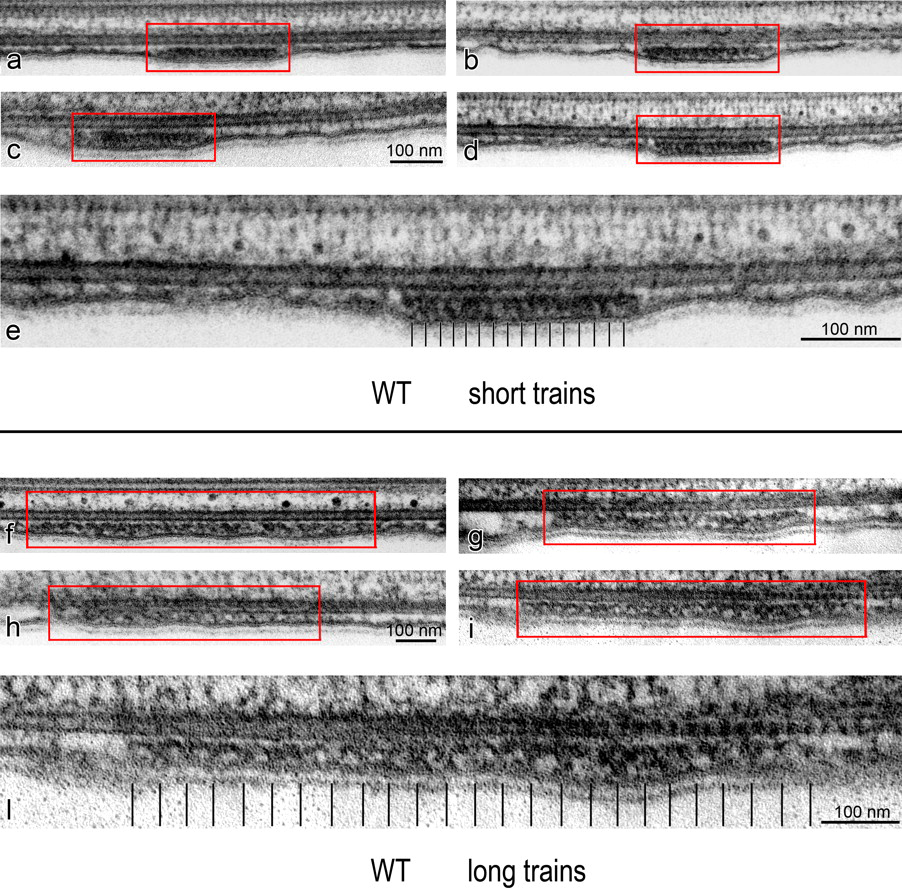
\includegraphics[width=\textwidth-60mm]{fig2-10.jpg}
%生成中英双语标题
{\setstretch{1.667}
\bicaption[fig:2.10]{图}{野生型衣藻鞭毛切片中的\ IFT\ 火车\ \citep{Pigino2009}。}{Figure}{TEM micrographs of \textit{in situ} IFT trains in flat-embedded flagella from  wild-type cells of \textit{Chlamydomonas reinhardtii} \citep{Pigino2009}.}
\par}
%结束图片浮动体环境
\end{figure}

IFT\ 复合物由\ IFT-B1、IFT-B2\ 和\ IFT-A\ 组成。其中\ IFT-A\ 中的外周亚基介导了\ IFT-A\ 核心复合物与\ IFT-B\ 之间的相互
作用\ \citep{Toriyama2016}。
2009\ 年,Pietro Lupetti\ 及其同事发现正向\ IFT\ 的长度为\ 700\ $\pm$\ 244 nm\ \citep{Pigino2009}
(图\ \ref{fig:2.10})。 这种长的\ IFT\ 火车实际上由两列火车平行组成,每列火车由颗粒状结构连接而成,其周期约\ 40 nm\ \citep{Pigino2009}。 正向\ IFT\ 沿\ B\ 管运动\ \citep{Pigino2009,Stepanek2016}。 反向\ IFT\ 的长度为\ 251\ $\pm$\ 45.1 nm,周期为\ \SI{16}{\nm},其结构致密,有极性\ \citep{Pigino2009} (图\ref{fig:2.10})。进一步研究表明,每一个微管二联管都是\ IFT\ 的双向二车道铁轨\ \citep{Stepanek2016}。 正向\ IFT\ 沿\ B\ 管从鞭毛基部移动到顶端,反向\ IFT\ 沿\ A\ 管从鞭毛顶端移动到基部\ \citep{Stepanek2016}。 这使得正向\ IFT\ 和反向\ IFT\ 在移动过程中不会出现碰撞。这一独特现象产生的原因可能是\ IFT\ 分子马达可识别\ A\ 管和\ B\ 管上不同的翻译后修饰\ \citep{Stepanek2016}。 也可能是由于在纤毛的基部和顶端存在特定机制可控制分子马达的轨道\
\citep{Stepanek2016}。然而,Pietro Lupetti\ 领导的团队在二零一六年发表的文章中修正了之前关于\ IFT\ 火车的模型\ \citep{Vannuccini2016}。他们在测定鞭毛再生过程中两种火车的相对数量时发现短火车的数量随鞭毛长度的增加而增加\ \citep{Vannuccini2016}。进一步的观测结果显示存在另一种更“致密”的短火车且与\ B\ 管的第七根原丝接触\ \citep{Vannuccini2016}。这表明存在两种类型的正向\ IFT\ 火车且它们的相对数量随纤毛形成的进行而变化\
\citep{Vannuccini2016}。

%开始图片浮动体环境,其中!表示取消严谨限制,h表示在此处插入,t表示在本页或下一页顶部插入
\begin{figure}[htb]
%居中对齐
\centering
%设置图片搜索路径,每个路径用{}括起来
\graphicspath{{figures/}}
%插入图片并设置图片宽度为文本宽度减10mm
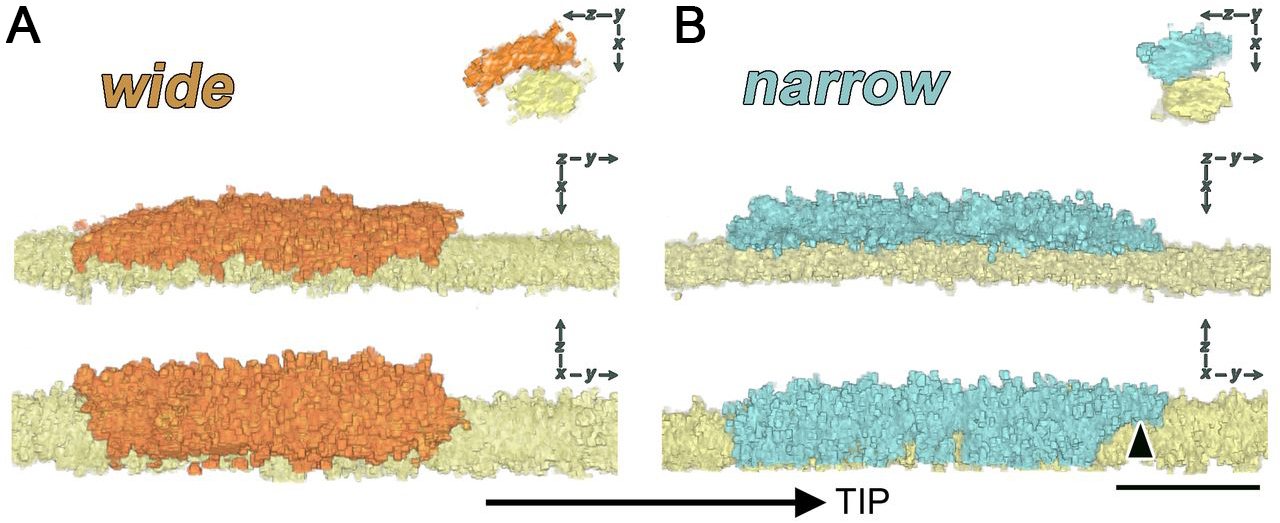
\includegraphics[width=\textwidth]{fig2-11.jpg}
%生成中英双语标题
{\setstretch{1.667}
\bicaption[fig:2.11]{图}{两种不同类型的短火车\ \citep{Vannuccini2016}。相比于较宽的一种(A),较窄的短火车(B)有一个指向鞭毛顶端的狭长凸起(黑色三角)。黄绿色结构为微管,红色和蓝色结构为\ IFT\ 火车。标尺代表\ \SI{100}{\nm}。}{Figure}{The two subtypes of short IFT trains \citep{Vannuccini2016}. Compared with the wide short train (A), there is a slender projection pointing toward the flagellar tip (black triangle) in the narrow short train (B). The flavogreen structures are microtubules. The red and blue structures are IFT trains. Scale bar represents \SI{100}{\nm}.}
\par}
%结束图片浮动体环境
\end{figure}

IFT\ 火车由\ IFT\ 复合物组成,IFT\ 复合物包含\ IFT-B1、IFT-B2\ 和\ IFT-A\ 三个亚复合物。在\ IFT-B1 \ 中,IFT88、 IFT70、IFT52\ 和\ IFT46\ 之间存在相互作用
(图\ \ref{fig:2.12}A)\citep{Taschner2014}。 其中\ IFT52/IFT46\ 两个亚基的\ C\ 端紧密结合形成球形结构域与\ IFT81/IFT74\ 相互作用(图\ \ref{fig:2.12}A)\citep{Taschner2014}。后者的\ C\ 端结合了\ IFT27/IFT25,N\ 端则为微管蛋白结合位点\ \citep{Bhogaraju2013a,Bhogaraju2014,Kubo2016}。在早期的研究中,IFT\ 复合物\ B\ 中的亚基被分为核心亚基和外周亚基。然而,最新的研究表明这些外周亚基可以形成稳定的复合物\ IFT-B2,它与核心复合物\ IFT-B1\ 之间的相互作用是由\ IFT88/IFT57/IFT52/IFT38\ 介
导(图\ \ref{fig:2.12}B)\citep{Taschner2016a}。 在\ IFT-B2\ 中,IFT54\ 的\ CH\ 结构域也可结合微管蛋白,而\ IFT38\ 的\ CH\ 结构域结合\ IFT80,IFT57\ 的\ CH\ 结构域则结合\ IFT172\ \citep{Taschner2016a}。 尽管纤毛是十分保守的细胞器,不同物种中\ IFT\ 的组成和结构可能存在微小的差异。在哺乳动物初级纤毛中,IFT56\ 与\ IFT46\ 存在相互作用,而\ IFT70\ 则仅与\ IFT88/IFT52\ 相互
作用(图\ \ref{fig:2.12}C)\citep{Katoh2016}。在外周亚基中,IFT57、IFT38\ 和\ IFT20\ 有形成同源二聚体的趋势\ \citep{Katoh2016}。
%开始图片浮动体环境,其中!表示取消严谨限制,h表示在此处插入,t表示在本页或下一页顶部插入
\begin{figure}[htb!p]
%居中对齐
\centering
%设置图片搜索路径,每个路径用{}括起来
\graphicspath{{figures/}}
%插入图片并设置图片宽度为文本宽度减10mm
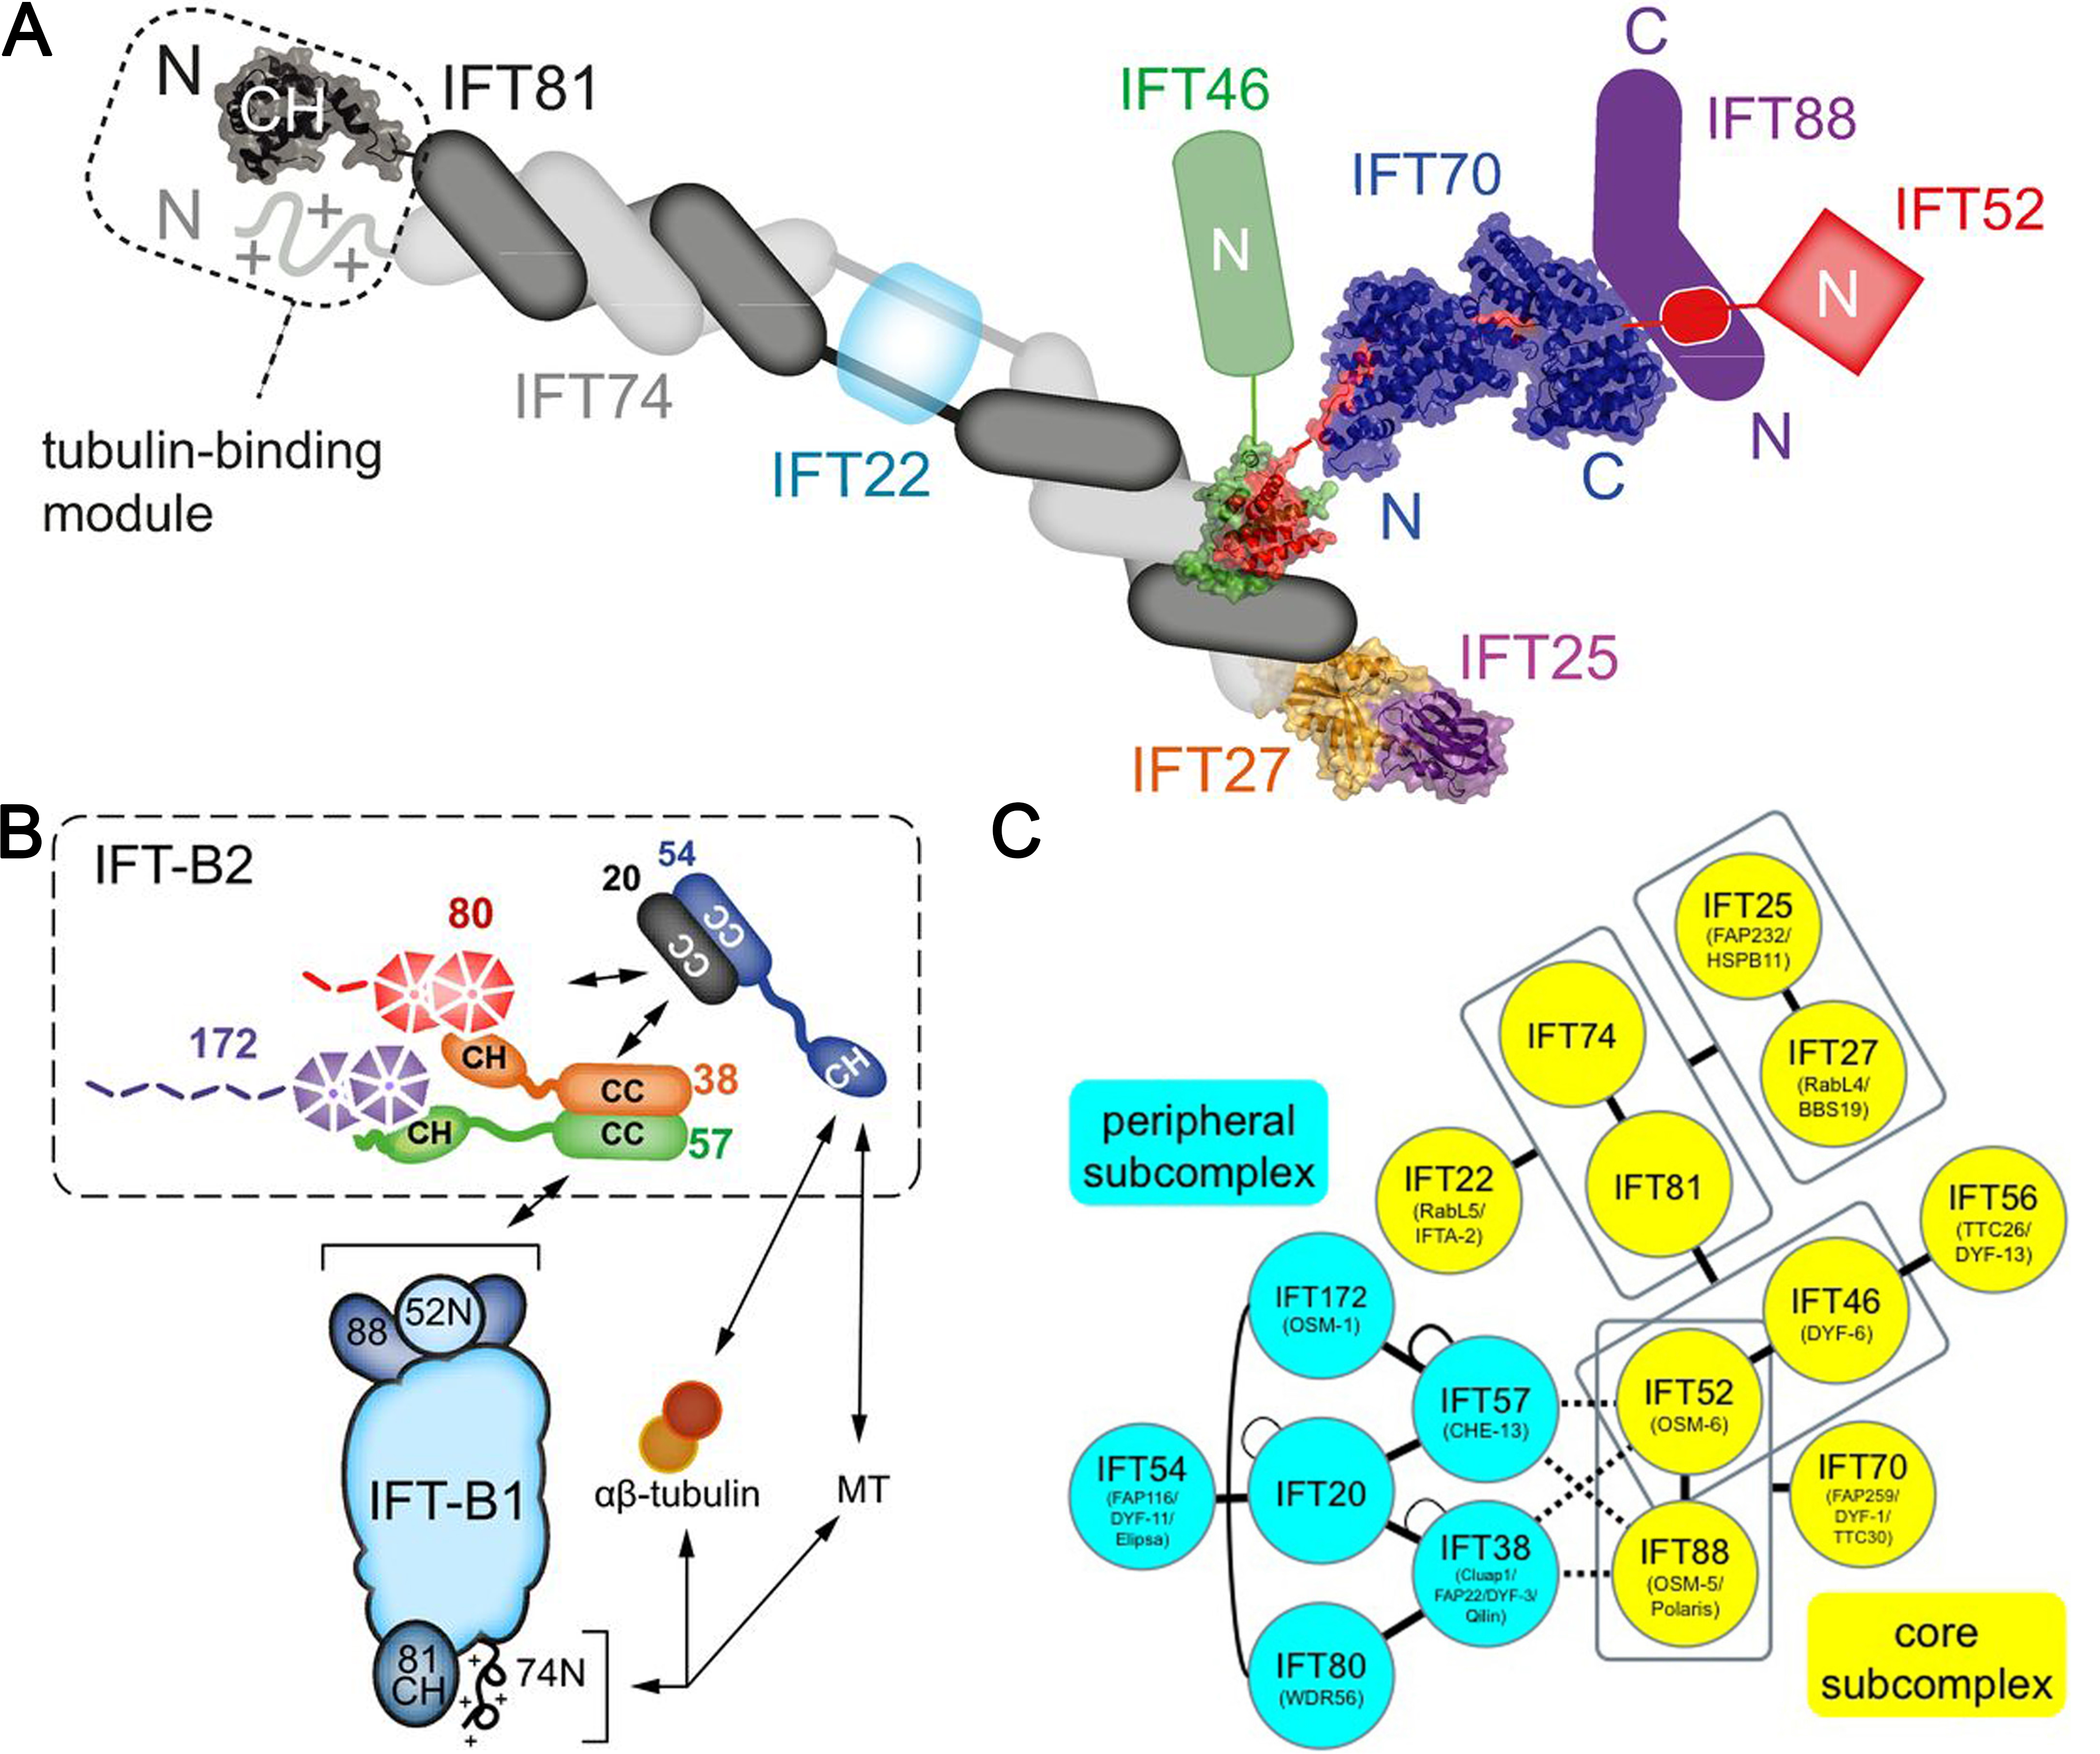
\includegraphics[width=\textwidth]{fig2-12.jpg}
%生成中英双语标题
{\setstretch{1.667}
\bicaption[fig:2.12]{图}{IFT\ 复合物\ B\ 的整体构造。(A)衣藻\ IFT-B\ 核心复合物的构
造\ \citep{Taschner2014}。其中\ IFT81\ 和\ IFT74\ 的\ N\ 端组成了微管结合模块负责微管蛋白的鞭毛内运输。(B)衣藻\ IFT-B1\ 与\ IFT-B2\ 的构造\ \citep{Taschner2016a}。图中将\ IFT54\ 的\ CH\ 结构域也标记为可能的围观蛋白/微管结合位点。(C)哺乳动物初级纤毛\ IFT-B\ 的整体构造\ \citep{Katoh2016}。 黑色粗线代表强相互作用,黑色细线代表弱相互作用,灰色曲线代表同源二聚体,灰色方框代表异源二聚体。}{Figure}{Architecture of the IFT-B complex. (A) Architecture of the core complex of IFT-B in \textit{Chlamydomonas} flagella \citep{Taschner2014}. The N terminuses of IFT81 and IFT74 form a tubulin-binding module which is responsible for the IFT of tubulin. (B) Overall architecture of the IFT-B1 and IFT-B2 complex in \textit{Chlamydomonas} flagella \citep{Taschner2016a}. The CH domain of IFT54 is also labeled as putative tubulin or MT binding site. (C) A map of interactions among IFT-B subunits in mammalian cilia \citep{Katoh2016}. Black thick lines represent strong interactions. Black fine lines represent weak interactions. Grey curved lines indicate homodimers. Grey boxes indicate heterodimers.}
\par}
%结束图片浮动体环境
\end{figure}

已鉴定的\ IFT\ 复合物\ A\ 亚基仅有六个,其中\ IFT144/IFT140/IFT122\ 被称为核心复合物,其余三个亚基则为外周亚基(图\ \ref{fig:2.13})。在核心复合物中,IFT122\ 是核心,而\ IFT121\ 则是外周亚基的组织
者\ \citep{Zhu2017}。IFT139\ 和\ IFT43\ 与核心复合物的连接依赖\ IFT121\ 与\ IFT122\ 之间的相互
作用(图\ \ref{fig:2.13})\citep{Behal2012}。在线虫神经元纤毛中,IFT139\ 和\ IFT43\ 在参与\ dynein-2\ 介导的反向\ IFT\ 的过程中存在功能冗余\ \citep{Yi2017}。这种情况是否普遍存在于反向\ IFT\ 有待进一步研究。实验结果表明,IFT43\ 与\ IFT121\ 的\ C\ 端可以发生直接相互
作用\ \citep{Behal2012}。 然而,在整个细胞体中仅有部分\ IFT43\ 与其他\ IFT\ 复合物\ A\ 的亚基聚合在一起,这表明\ IFT43\ 可能还有其他未知的功能\ \citep{Behal2012,Zhu2017}。

%开始图片浮动体环境,其中!表示取消严谨限制,h表示在此处插入,t表示在本页或下一页顶部插入
\begin{figure}[htb]
%居中对齐
\centering
%设置图片搜索路径,每个路径用{}括起来
\graphicspath{{figures/}}
%插入图片并设置图片宽度为文本宽度减10mm
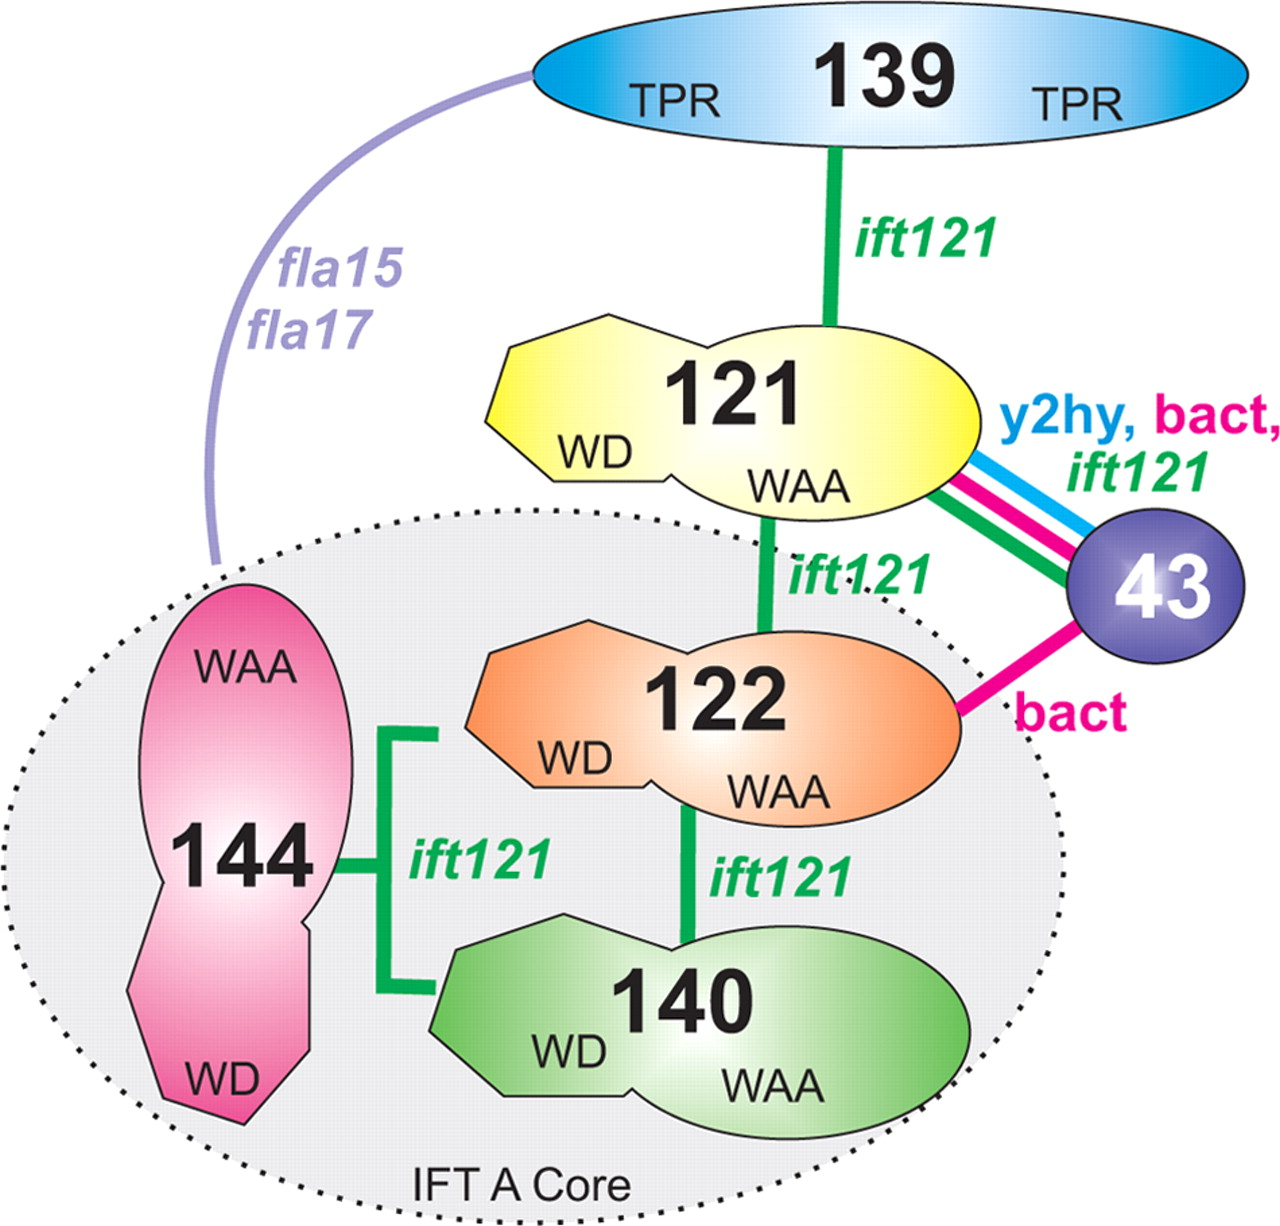
\includegraphics[width=\textwidth-60mm]{fig2-13.jpg}
%生成中英双语标题
{\setstretch{1.667}
\bicaption[fig:2.13]{图}{IFT\ 复合物\ A\ 中各亚基之间的相互作用网络\ \citep{Behal2012}。对突变
体\ \textit{ift121}\ 进行的分析表明\ IFT122、IFT140\ 和\ IFT144\ 组装成异源三聚体形成\ IFT\ 复合物\ A\ 的核心。由于\ IFT121\ 的突变可导致复合物\ A\ 中\ IFT139\ 和\ IFT43\ 的完全缺失,我们认为\ IFT121\ 与二者均存在相互作用。} {Figure}{A map of interactions among IFT-B subunits \citep{Behal2012}. Based on biochemical analysis of the \textit{ift121} mutant, we propose that IFT122, IFT140, and IFT144 assemble to create a heterotrimeric stable core complex. The interactions of IFT121 with both IFT139 and IFT43 are supported by the observation that loss of IFT121 completely removes IFT139 and IFT43 from complex A.}
\par}
%结束图片浮动体环境
\end{figure}

\section{纤毛蛋白定位相关研究}
\subsection{纤毛扩散屏障及纤毛孔复合物}
\subsubsection{纤毛扩散屏障}
纤毛是突出在细胞表面的细胞器,其内部空间与胞质空间是一体的。胞质组分从胞浆进入纤毛是否受到限制是一个重要的问题。换句话说,是否存在纤毛扩散屏障或类似核孔复合物的控制物质进出纤毛的结构?

%开始图片浮动体环境,其中!表示取消严谨限制,h表示在此处插入,t表示在本页或下一页顶部插入
\begin{figure}[htbp!]
%居中对齐
\centering
%设置图片搜索路径,每个路径用{}括起来
\graphicspath{{figures/}}
%插入图片并设置图片宽度为文本宽度减10mm
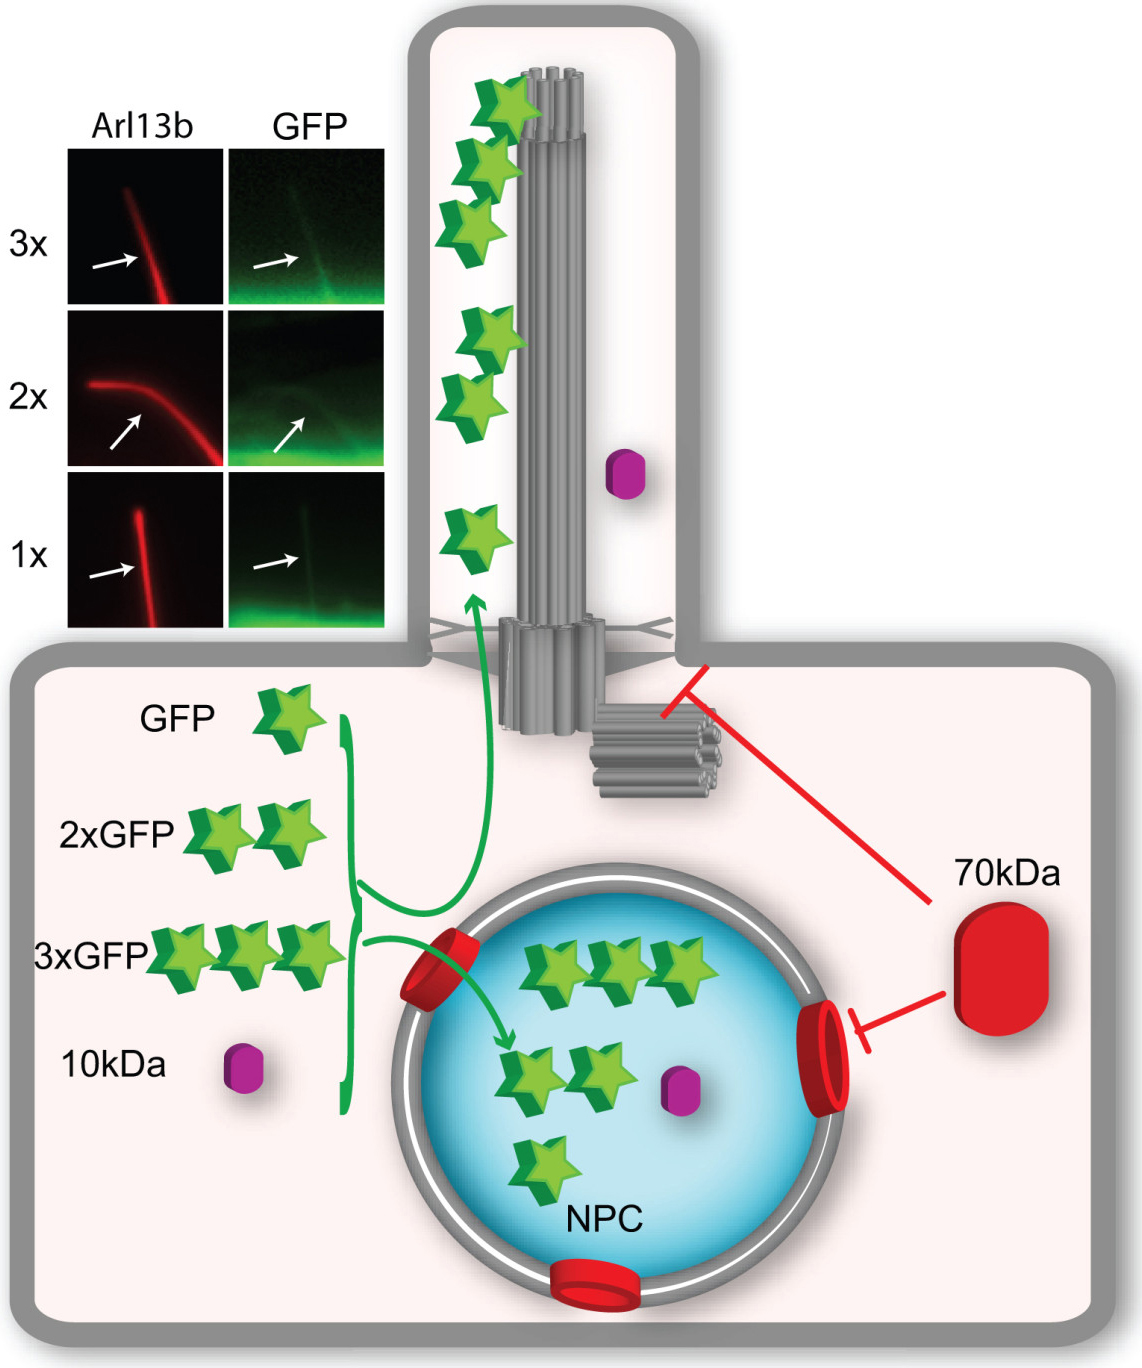
\includegraphics[width=\textwidth-50mm]{fig2-3.jpg}
%生成中英双语标题
{\setstretch{1.667}
\bicaption[fig:2.3]{图}{纤毛基部分子大小依赖的扩散屏障模型\ \citep{Kee2013}。 纤毛基部存在分子大小依赖的扩散屏障用于控制可溶性蛋白进入纤毛。10 kDa\ 的分子(紫色)能够自由出入纤毛和细胞核,但\ 70 kDa\ 的分子(红色)则受到限制。左上角插入的图片为\ NIH3T3\ 细胞的纤毛,红色为纤毛标记物\ Arl13b,绿色为\ GFPs\ 或串联\ GFPs。 尽管\ GFPs\ 和串联\ GFPs\ 的分子量存在差异,但它们均能够进入纤毛。这可能是由于二者具有相似的分子直径。GFP\ 代表绿色荧光蛋白,NPC\ 代表核孔复合物。}{Figure}{Model of the size-dependent diffusion barrier at the base of the cilium
\citep{Kee2013}. The base of the cilium contains a size-dependent barrier to entry of soluble proteins. Molecules that are 10 kDa (purple) can enter both the cilium and nucleus but 70 kDa (red) molecules are restricted from both compartments. Insets shows fluorescence micrographs of the cilia of NIH3T3 cells co-expressing monomeric GFP (1x) or tandem (2x or 3x) GFPs together with Arl13b (red) to mark the ciliary compartment. Despite the difference in molecular weight, monomeric and tandem fluorescent protein constructs can enter the ciliary compartment, presumably due to their similar diameters. GFP, green fluorescent protein; NPC, nuclear pore complexes.}
\par}
%结束图片浮动体环境
\end{figure}

Calvert\ 及其同事发现爪蟾感光细胞的连接纤毛(等同于常规纤毛的转变区)不能有效阻止绿色荧光蛋白在内节和外节之间扩散\ \citep{Calvert2010}(图\ \ref{fig:2.3})。进一步研究发现串联绿色荧光蛋白(2x 和3x)也能够通过连接纤毛自由扩散\
\citep{Najafi2012}。 据此,Calvert\
等人认为纤毛基部不存在控制物质出入的扩散屏障(至少对小于\ 80 kDa\ 的蛋白来
说是这样)\citep{Najafi2012}。

然而在哺乳动物细胞初级纤毛上的研究却得出了相反的结论。研究人员将不同分子量的荧光葡聚糖注射到细胞内并观察它们的运动\ \citep{Kee2012}。结果显示小于\ 10 kDa\ 的荧光葡聚糖能够进入细胞核和纤毛,而\ 40-70 kDa\ 的荧光葡聚糖却无法进入\ \citep{Kee2012}。使用荧光标记的可溶性蛋白进行的实验也获得了同样的结果\ \citep{Kee2013}。 这些研究表明大于\ 50 kDa\ 的蛋白无法通过自由扩散进入纤毛,它们的运动受到纤毛扩散屏障的限制\ \citep{Kee2013}。

这些矛盾出现的可能原因是由于在爪蟾中使用的串联绿色荧光蛋白是线性的,而在初级纤毛中使用的葡聚糖和可溶性蛋白是球形的\ \citep{Kee2013}。这意味着纤毛扩散屏障对出入的蛋白的大小和空间结构均存在限制。这一假说已被相关研究证实\ \citep{Kee2013,Lin2013}。总之,纤毛基部存在基于分子大小的扩散屏障,它能有效控制物质出入纤毛
(图\ \ref{fig:2.3})。

\subsubsection{纤毛孔复合物}
纤毛扩散屏障的分子组成是什么呢?核孔蛋白是组成核孔复合物的一类蛋白,研究表明某些核孔蛋白定位在初级纤毛基部形成纤毛孔复合物(ciliary pore complex, CPC)\ \citep{Kee2012,Diener2015}。分子马达\ KIF17\ 进入纤毛依赖这些核孔蛋白的作
用\ \citep{Kee2012}。 这表明纤毛扩散屏障和核孔共享某些分子组分。然而纤毛孔复合物在组成上与核孔复合物可能并非完全一致。这是因为某些关键的核孔蛋白并未出现在纤毛基部,比如核篮亚复合物中的负责细胞核特异性平台形成的核孔蛋白和将\ NPC\
锚定在核膜上的跨膜核孔蛋白\ \citep{Kee2012}。尽管后者的功能可以由纤毛基部的\ NPHK/MKS\ 复合物执行\ \citep{Garcia-Gonzalo2012},这些差异表明\ CPC\ 可能使用了与\ NPC\ 不完全相同的结构蛋白和控制机制\ \citep{Kee2012}。

%开始图片浮动体环境,其中!表示取消严谨限制,h表示在此处插入,t表示在本页或下一页顶部插入
\begin{figure}[htb!]
%居中对齐
\centering
%设置图片搜索路径,每个路径用{}括起来
\graphicspath{{figures/}}
%插入图片并设置图片宽度为文本宽度减10mm
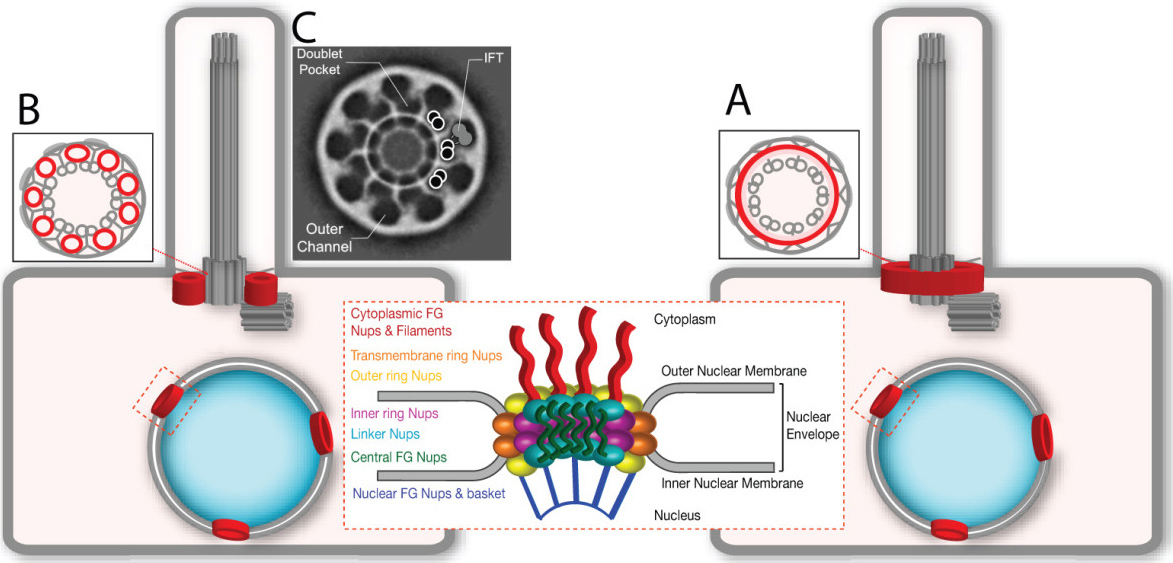
\includegraphics[width=\textwidth]{fig2-4.jpg}
%生成中英双语标题
{\setstretch{1.667}
\bicaption[fig:2.4]{图}{纤毛和细胞核中的核孔蛋白。核孔复合物由一系列的核孔蛋白组成,其中部分核孔蛋白也定位在纤毛基体形成纤毛孔复合物\ \citep{Kee2013}。图中展示了纤毛孔复合物两种可能的结构。(A)核孔蛋白在纤毛基部形成一个大的纤毛孔,轴丝从纤毛孔的中央突出延伸。(B)核孔蛋白在\ Y-links\ 之间形成九个纤毛孔。(C)梨形四膜虫纤毛基体的电镜照片显示在轴丝外围有九个孔
状结构\ \citep{Ounjai2013}。}{Figure}{Nucleoporins in cilia and nuclei. Nuclear pore complexes contain nucleoporin proteins that assemble into subcomplexes \citep{Kee2013}. Some nucleoporin subcomplexes also localize to the transition zone where they are postulated to form a ciliary pore complex. Two possible structural configurations of the nucleoporins at the base of the cilium are presented. (A) Model in which nucleoporins assemble into one large pore at the base of the cilium with the axoneme protruding through the middle of the pore. (B) Model in which nucleoporins assemble into nine pores at the base of the cilium with each pore positioned between the Y-links. (C) Electron cryotomography analysis of isolated basal body structures from the protist \textit{Tetrahymena pyriformis} indicates nine pore structures adjacent to the microtubule axonemes
\citep{Ounjai2013}.}
\par}
%结束图片浮动体环境
\end{figure}

关于\ CPC\ 的另一个重要问题与其整体结构有关。每一个\ NPC\ 都具有典型的\ 8\ 次旋转对称
结构\ \citep{Alber2007},而纤毛确是\ 9+(0)\ 或\ 9+(2)\ 结构\ \citep{Czarnecki2012}。由于我们对核孔蛋白如何在纤毛基部组装形成\ CPC\ 一无所知,这种对称性的差异是否具有重要意义也
不得而知\ \citep{Kee2013}。 一种可能性是核孔蛋白在纤毛基部形成一个大孔,轴丝从孔中穿过(图\ref{fig:2.4})。这样的纤毛孔具有\ 9\ 次旋转对称结构\ \citep{Kee2013}。另一种可能性是在\ Y\ 型连接结构中间有九个纤毛孔(图\ \ref{fig:2.4}),这样的纤毛孔将具有核孔的八次旋转对称结构\ \citep{Kee2013}。 以嗜热四膜虫纤毛为对象进行的研究支持后一种假说\
\citep{Ounjai2013}。研究人员在嗜热四膜虫鞭毛基体中观察到九个靠近轴丝二联管的孔状结构,其直径约\ 53 nm\
\citep{Ounjai2013}。 这与核孔的直径非常接近\ \citep{Beck2004}。此外,研究人员还从分离的基体中鉴定到参与核- 胞质转运的蛋白如\ Ran\
和跨膜核孔蛋白\ NDC-1\ \citep{Ounjai2013}。这些结果进一步表明\ CPC\ 与\ NPC\ 之间存在相似性。

\subsection{纤毛定位序列}
纤毛中的结构和功能蛋白如何被纤毛蛋白运输系统识别并招募到纤毛呢?对纤毛蛋白的研究显示存在特殊的信号序列即纤毛定位序列(ciliary targeting sequence, CTS)将它们靶定到纤毛\ \citep{Malicki2014}。在跨膜蛋白中,CTS\
一般出现在膜的胞质侧(无论是在胞内囊泡还是在纤毛膜上)\citep{Malicki2014}。CTS\ 一般在蛋白的\ C
\ 端,极少出现在\ N\
端,但有时会出现在多重跨膜蛋白的胞内环上\ \citep{Laird2015}。CTS\ 具有多样性,这意味着它们会与不同的运输系统互作\ \citep{Malicki2014}。研究表明,多个信号通路参与了蛋白的纤毛定位。尽管到目前为止大多数\ CTS\ 的结合对象仍然未知,但对纤毛定位序列的研究已经取得了一系列成果并将持续产生有价值的信息。

\subsubsection{RVxP\ 基序}
最常见的\ CTS\ 是\ RVxP\ 基序,目前只在跨膜蛋白和膜相关蛋白中鉴定到,比如\ G\ 蛋白偶联受体、多囊蛋白\ 2、 环核苷酸 门控离子通道蛋白\ CNGB1b、钠钾腺苷三磷酸酶和视黄醇脱氢酶等\
\citep{Laird2015,Geng2006,Jenkins2006,Michalakis2006}。 其中多囊蛋白\ 2\
的\ RVxP\
基序位于\ N\
端,包含该基序的\ N\
端可将人转铁蛋白受体\ hTFR\ 定位到纤毛\ \citep{Geng2006}。

在实验条件下,RVxP\ 基序通常是蛋白靶定到纤毛所必须的,其突变可破坏蛋白的纤毛定位。以人视杆细胞视蛋白为例,其\ RVxP\ 基序的突变可导致视网膜光受体细胞损伤,这是由视蛋白在细胞体中的异位累积导致的\ \citep{Tam2000}。然而,并非所有纤毛蛋白\ C\ 端的\ RVxP\ 基序都是有功能的。比如纤毛肌醇多聚磷酸磷酸酶\ Inpp5e\ 的\ C\ 端\ RVxP\ 基序突变并不影响其纤毛定位。

视蛋白的\ RVxP\ 基序是其靶定到纤毛所必须的,但其他特征序列的存在也必不可少\ \citep{Tam2000}。视蛋白\ C\ 端\ 44\ 个氨基酸残基组成的多肽(视蛋白\ C44)含有\ RVxP\ 基序,它可以将外源蛋白如\ GFP\ 靶定到纤毛。这依赖视蛋白\ C44\ 与膜相互作用,而这与两个相邻的半胱氨酸残基的棕榈酰化有关。它们的缺失将造成视蛋白无法定位到纤毛,且其表型比\ RVxP\ 基序的突变导致的更严重。这些研究表明在光受体细胞中与膜相互作用对蛋白靶定到纤毛至关重要\ \citep{Laird2015}。
多个研究小组通过蛋白质组学的方法鉴定了一些与视蛋白\ C44\ 相互作用的蛋白。生化分析表明这些蛋白作用于视蛋白纤毛定位过程的不同阶段\ \citep{Tam2000,Laird2015}。其中鸟苷三磷酸酶\ Arf4\ 可以结合视蛋白的\ CTS\ 从而介导囊泡从\ TGN\ 上出芽,这是视蛋白纤毛定位的起始过程。最新的研究表明\ Arf4\ 可以增强\ ASAP1\ 与\ FR\ 模体的结合。这反过来可以起始\ Rab11/Rabin8/Rab8\ 复合物的组装。后者可引发视蛋白转位到纤毛。酵母双杂交筛选显示视蛋白的\ C\ 端与胞质动力蛋白存在直接相互作用,研究人员据此推测视蛋白的纤毛定位是依赖微管的。

嗅觉感受神经元纤毛上的环核苷酸门控离子通道蛋白\ CNGB1b\ 的\ C\ 端也含有\ RVxP\ 基序\ \citep{Jenkins2006}。 该蛋白对环核苷酸门控离子通道复合物的纤毛定位是必须的\ \citep{Jenkins2009,Michalakis2006}。 进一步研究发现胞内分选蛋白\ PACS-1\
通过直接结合\ CNGB1b\ 并决定其纤毛定位\ \citep{Jenkins2009}。二者的相互作用依赖丝氨酸/苏氨酸蛋白激酶\ CK2\ 对它们的磷酸化修饰\ \citep{Jenkins2009}。

\subsubsection{FR\ 基序及\ I3-CTS}
除了\ RVxP\ 基序和棕榈酰化的残基外,视蛋白\ C44\ 还含有\ FR\ 基序(其功能暂时没有被证实)。该基序最早在线虫嗅觉\ G\ 蛋白偶联受体\ ODR-10\ 上发现\ \citep{Dwyer2001},其他\ G\ 蛋白偶联受体的\ C\ 端也有该基序。它含有一个疏水氨基酸残基和一个碱性氨基酸残基。FR\ 基序的突变可导致\ ODR-10\ 和\ Smoothened (Smo)\ 无法靶定到纤毛\ \citep{Dwyer2001}。除\ RVxP\ 基序外,许多\ G\ 蛋白偶联受体在它们的第三个胞内环上有纤毛定位序列(I3-CTS)\citep{Berbari2008}。比如生长抑素受体\ SSTR3\ 在该区域含有\ Ax[S/A]xQ\ 基序\ \citep{Berbari2008}。大鼠中枢神经系统中的其他五个生长抑素受体没有该基序,它们也不定位在纤毛。结构域嵌合实验表明\ I3-CTS\ 基序具有重要作用。含有\ SSTR3\ 的\ I3-CTS\ 的\ SSTR5\ 可以定位到纤
毛\ \citep{Berbari2008}。Ax[S/A]xQ\ 基序的突变可破坏该嵌合蛋白的纤毛定位。同样的结论在血清素受体\ HTR6\ 和黑色素浓集激素受体\ MCHR1\
上也得到证实\ \citep{Berbari2008}。然而,并非所有的\ I3-CTS\ 都具有关联。如神经肽\ Y\ 受体\ NPY2R\ 的两个\ I3-CTS\ 与\ SSTR3\ 的就没有相似性。

与视蛋白不同,GPCR\ 的纤毛定位依赖\ I3-CTS,其功能的实现可能由\ BBS\ 蛋白复合体
介导\ \citep{Berbari2008a}。 在小鼠中敲除\ BBS2\ 和\ BBS4\ 可破坏\ SSTR3\ 和\ MCHR1\ 的纤毛定位\ \citep{Berbari2008a}。同样,在培养的细胞中干扰\ BBS3\ 和\ BBS4\ 会影响含有\ SSTR3 I3-CTS\ 的嵌合跨膜蛋白的纤毛定位\ \citep{Berbari2008a}。 在蛋白相互作用的研究中,SSTR3\ 的\ I3-CTS\ 可以“捕获”所有检测的\ BBSome\ 亚基,而多巴胺受体\ 1\ 则与\ BBS5\ 存在直接相互作用\ \citep{Berbari2008a}。总而言之,I3-CTS\ 的功能可能是使\ GPCR\ 与\ BBS\ 蛋白形成的膜外壳连成一体\ \citep{Berbari2008a}。

除\ BBS\ 蛋白外,肥胖相关蛋白\ TULP3\ 和\ IFT\ 复合物\ A\ 对\ SSTR3\ 和\ MCHR1\ 的纤毛定位也有贡献。TULP3\ 依赖其\ N\ 端与\ IFT\ 复合物\ A\ 发生相互作用\ \citep{Mukhopadhyay2010}。而\ IFT\ 复合物\ A\ 和\ TULP3\ 又反过来共同调控了\ SSTR3\ 和\ MCHR1\ 的纤毛定位\ \citep{Mukhopadhyay2010}。 其中,TULP3\ 与\ IFT\ 复合物\ A\ 及磷脂酰肌醇的结合对调控功能的发挥是必须的\
\citep{Mukhopadhyay2010}。

理论上,不同纤毛定位序列通过不同的途径发挥作用。然而这些通路的上游可能是同种因子,比如肥胖相关蛋白\ Tubby。 尽管视蛋白和\ GPCRs\ 的\ CTS\ 存在差异,肥胖相关蛋白\ Tubby\ 却对视蛋白、生长抑素受体\ SSTR3\ 和黑色素浓集激素受体\ MCHR1\ 的纤毛定位均起到调控作用\ \citep{Sun2012}。在\ tubby\ 突变小鼠的视网膜中,视蛋白无法完全穿过连接纤毛到达外段\
\citep{Sun2012}。 而\ SSTR3\ 和\ MCHR1\ 则无法正确定位到大脑神经元的初级纤毛中发挥功能\citep{Sun2012}。

\subsubsection{核定位信号}
研究表明纤毛扩散屏障与核孔复合物之间存在一定的相似性\ \citep{Huang2010}。研究人员将这种类似核孔复合物的结构称之为纤毛孔复合物\ \citep{Kee2013}。这意味着核定位信号(nuclear localization signal, NLS)及相关蛋白可能同时也参与蛋白的纤毛定位\ \citep{Huang2010}。

KIF17\ 是一种正向\ IFT\ 分子马达,正常情况下它定位在纤毛顶端。其\ C\ 端的\ CTS\ 是一连串碱性氨基酸残基组成的多肽,与经典核定位信号存在相似性\ \citep{Dishinger2010}。缺失该\ CTS\ 的\ KIF17\ 无法定位到纤毛。该\ CTS\ 在单独表达的情况下可以定位在细胞核和纤毛。进一步的研究表明\ KIF17\ 的\ CTS\ 通过与\ importin-$\upbeta$2\ 相互作用发挥纤毛定位的功能\
\citep{Dishinger2010}。

视网膜色素\ RP2\ 是一种脂锚定外周膜蛋白\ \citep{Hurd2011}。其氨基酸序列中含有经典及非经典\ NLS。 突变分析发现\ RP2\ 的非经典\ NLS\ 对其纤毛定位至关重要\ \citep{Hurd2011}。该非经典\ NLS\ 通过结合\ importin-$\upbeta$2\ 介导\ RP2\ 通过纤毛孔复合物\
\citep{Hurd2011}。 电压门控性钾离子通道蛋白\ Kv10.1\ 定位在中心体和纤毛膜上调控纤毛解聚,其\ C\ 端含有\ NLS\
\citep{Sanchez2016,Chen2011}。研究表明该\ NLS\ 对\ Kv10.1\ 的纤毛定位至关重要\
\citep{Sanchez2016}。此外,importin-$\upbeta$1\ 被发现能够与纤毛膜蛋白\ Crumbs\ 结合\ \citep{Fan2007}。 然而它们之间的相互作用是否调控了\ Crumbs\ 的纤毛定位还有待进一步研究\citep{Fan2007}。

\subsubsection{类泛素化修饰}
由于调控蛋白进入细胞核和纤毛的结构存在相似之处,控制蛋白入核的其他机制很可能在蛋白进入纤毛的过程中也发挥作用。类泛素化修饰\ SUMOylation\ 是除\ NLS\ 之外的一种广泛存在的控制蛋白入核的方式\
\citep{Zhang2002,Chen2006}。SUMO\footnote{small ubiquitin-related modifier}\ 是一类重要的类泛素蛋白,其三维结构及生化修饰过程与泛素类似,但这两类蛋白质修饰的生物学意义却不尽相同\ \citep{Hay2005}。 研究表明这种翻译后修饰在腺苷酸环化酶\ AC3\
进入纤毛的过程中发挥重要作用\ \citep{McIntyre2015}。腺苷酸环化酶\ AC3\ 定位在神经元纤毛的膜上,常被用作神经元纤毛标记蛋白\ \citep{Bishop2007}。对\ AC3\ 的生物信息学分析显示其含有保守的类泛素化基序
\ \citep{McIntyre2015}。 进一步研究表明\ AC3\ 是类泛素化蛋白的底物\ \citep{McIntyre2015}。 抑制类泛素化修饰系统不影响纤毛的形成与维持,但\ AC3\
无法定位在纤毛\ \citep{McIntyre2015}。同样的,类泛素化基序突变的\ AC3\
也无法定位到纤毛\ \citep{McIntyre2015}。 这些结果表明类泛素化修饰对\ AC3\ 的纤毛定位非常重要。然而将\ AC3\
的类泛素化基序连接到非纤毛蛋白\ ANO1\
上并不能使\ ANO1\
定位到纤毛\ \citep{McIntyre2015}。这表明类泛素化修饰是\ AC3\
定位到纤毛的必要但不充分条件。

\subsection{IFT\ 蛋白基体定位相关研究}
\subsubsection{调控\ IFT\ 蛋白基体定位的蛋白质}
目前关于\ IFT\ 蛋白基体定位机制的研究较少。大部分研究集中在\ IFT20\ 上。然而,IFT20\ 大量聚集在高尔基体。该蛋白除参与纤毛的组装与解聚外还与蛋白转运等密切相关\ \citep{Follit2006,Follit2008}。 因而相关研究可能无法拓展到其他\ IFT\ 蛋白上。

免疫共沉淀实验显示\ IFT20\ 与\ CCDC41(Cep83)之间存在相互作用,CCDC41\ 对\ IFT20\ 被招募到中心体是必须的\
\citep{Joo2013}。此外,IFT20\ 离开顺式高尔基体膜囊受\ VPS15\ 和\ GM130\ 的调控\ \citep{Stoetzel2016}。VPS15\ 的突变导致\ IFT20\
无法有效从顺式高尔基体上释放从而造成纤毛变短\ \citep{Stoetzel2016}。然而,CCDC41\
并没有参与\ IFT88\
富集在中心体的过程\ \citep{Joo2013}。 由于\ IFT20\
和\ CCDC41\
参与纤毛囊泡的锚定而不是轴丝的延伸,故\ CCDC41\ 对\ IFT\
蛋白基体定位的调控可能不存在普遍性。与之类似,另一个与初级纤毛囊泡形成有关的蛋白\ EHD1\
对\ IFT20\
被招募到母中心粒远端也可能没有普遍性\ \citep{Lu2015,Naslavsky2011}。

在初级纤毛中,C2cd3\ 可以招募\ CCDC41、Cep164、TTBK2、IFT88\ 和\ IFT52\ 定位到母中心粒远端\
\citep{Ye2014,Cajanek2014},而\ TTBK2\ 可以招募\ IFT140\ 和\ IFT88\ 定位到过
渡区\ \citep{Goetz2012,Tsang2013}。OFD1\ 也可以招募\ IFT88\ 定位到基体\ \citep{Singla2010}。由于相关蛋白的抗体和突变体有限,以上关于\ IFT\ 蛋白基体定位的研究均比较零散。2016\ 年,Toriyama\ 及其同事发现纤毛病相关蛋白\ Jbts17(也被称为C5orf42)定位在基体,它可以招募\ CPLANE(包括Intu、Rsg1、Wdpcp、Jbts17\ 和\ Fuz)的其他成员定位到基体\
\citep{Toriyama2016}。CPLANE\
可以进一步招募\ IFT\ 复合物\ A\ 中的外周亚基定位到基体\ \citep{Toriyama2016}。2017\ 年,Yeyati\ 等人发现组蛋白赖氨酸去甲基化酶\ KDM3A\ 可通过调控肌动蛋白细胞骨架间接影响\ IFT\ 蛋白的基体和纤毛定
位\ \citep{Yeyati2017}。然而,目前还没有鉴定到直接影响\ IFT-A\ 核心亚基以及\ IFT-B\ 亚基基体定位的蛋白。

\subsubsection{IFT\ 蛋白基体定位相关模型}
纤毛内部无蛋白合成系统,纤毛延伸过程中其所需的前体蛋白均来自细胞体。研究表明,细胞体中存在纤毛前体蛋白的库\ \citep{Fowkes1998,Rosenbaum1969}。在衣藻中,这个库足够形成两根长度减半的鞭毛\
\citep{Rosenbaum1969}。 大部分纤毛蛋白在库中不是单个的存在,而是预组装形成复合物,如\ ODA\  \citep{Fowkes1998}、IDA\ \citep{Piperno1997}和\ RS\ \citep{Qin2004}。结合其他鞭毛蛋白基体定位机制的研究,“预组装-定位”可能是鞭毛蛋白基体定位的主要模式。

%开始图片浮动体环境,其中!表示取消严谨限制,h表示在此处插入,t表示在本页或下一页顶部插入
\begin{figure}[hbt]
%居中对齐
\centering
%设置图片搜索路径,每个路径用{}括起来
\graphicspath{{figures/}}
%插入图片并设置图片宽度为文本宽度减10mm
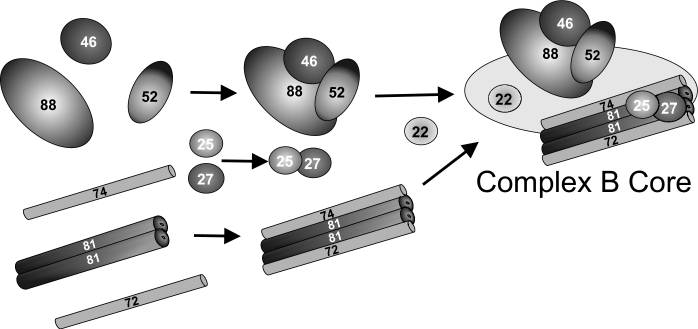
\includegraphics[width=\textwidth-40mm]{fig2-14.jpg}
%生成中英双语标题
{\setstretch{1.667}
\bicaption[fig:2.14]{图}{IFT-B\ 核心复合物体内组装的假想模型\ \citep{Lucker2010}。
IFT46、IFT52\ 和\ IFT88\ 形成异源三聚体并与\ IFT81、IFT74/72\ 异源四聚体和\ IFT27/25\ 异源二聚体组装。这些亚基或亚复合物组装的具体顺序是未知的。} {Figure}{Hypothetical model of \textit{in vivo} assembly of the IFT complex B core \citep{Lucker2010}. IFT46, IFT52, and IFT88 form a ternary complex prior to assembly with the IFT81, IFT74/72 tetramer and IFT27/25 heterodimer. The actual order in which these and additional subunits assemble onto the core is unknown.}
\par}
%结束图片浮动体环境
\end{figure}

%开始图片浮动体环境,其中!表示取消严谨限制,h表示在此处插入,t表示在本页或下一页顶部插入
\begin{figure}[htbp]
%居中对齐
\centering
%设置图片搜索路径,每个路径用{}括起来
\graphicspath{{figures/}}
%插入图片并设置图片宽度为文本宽度减10mm
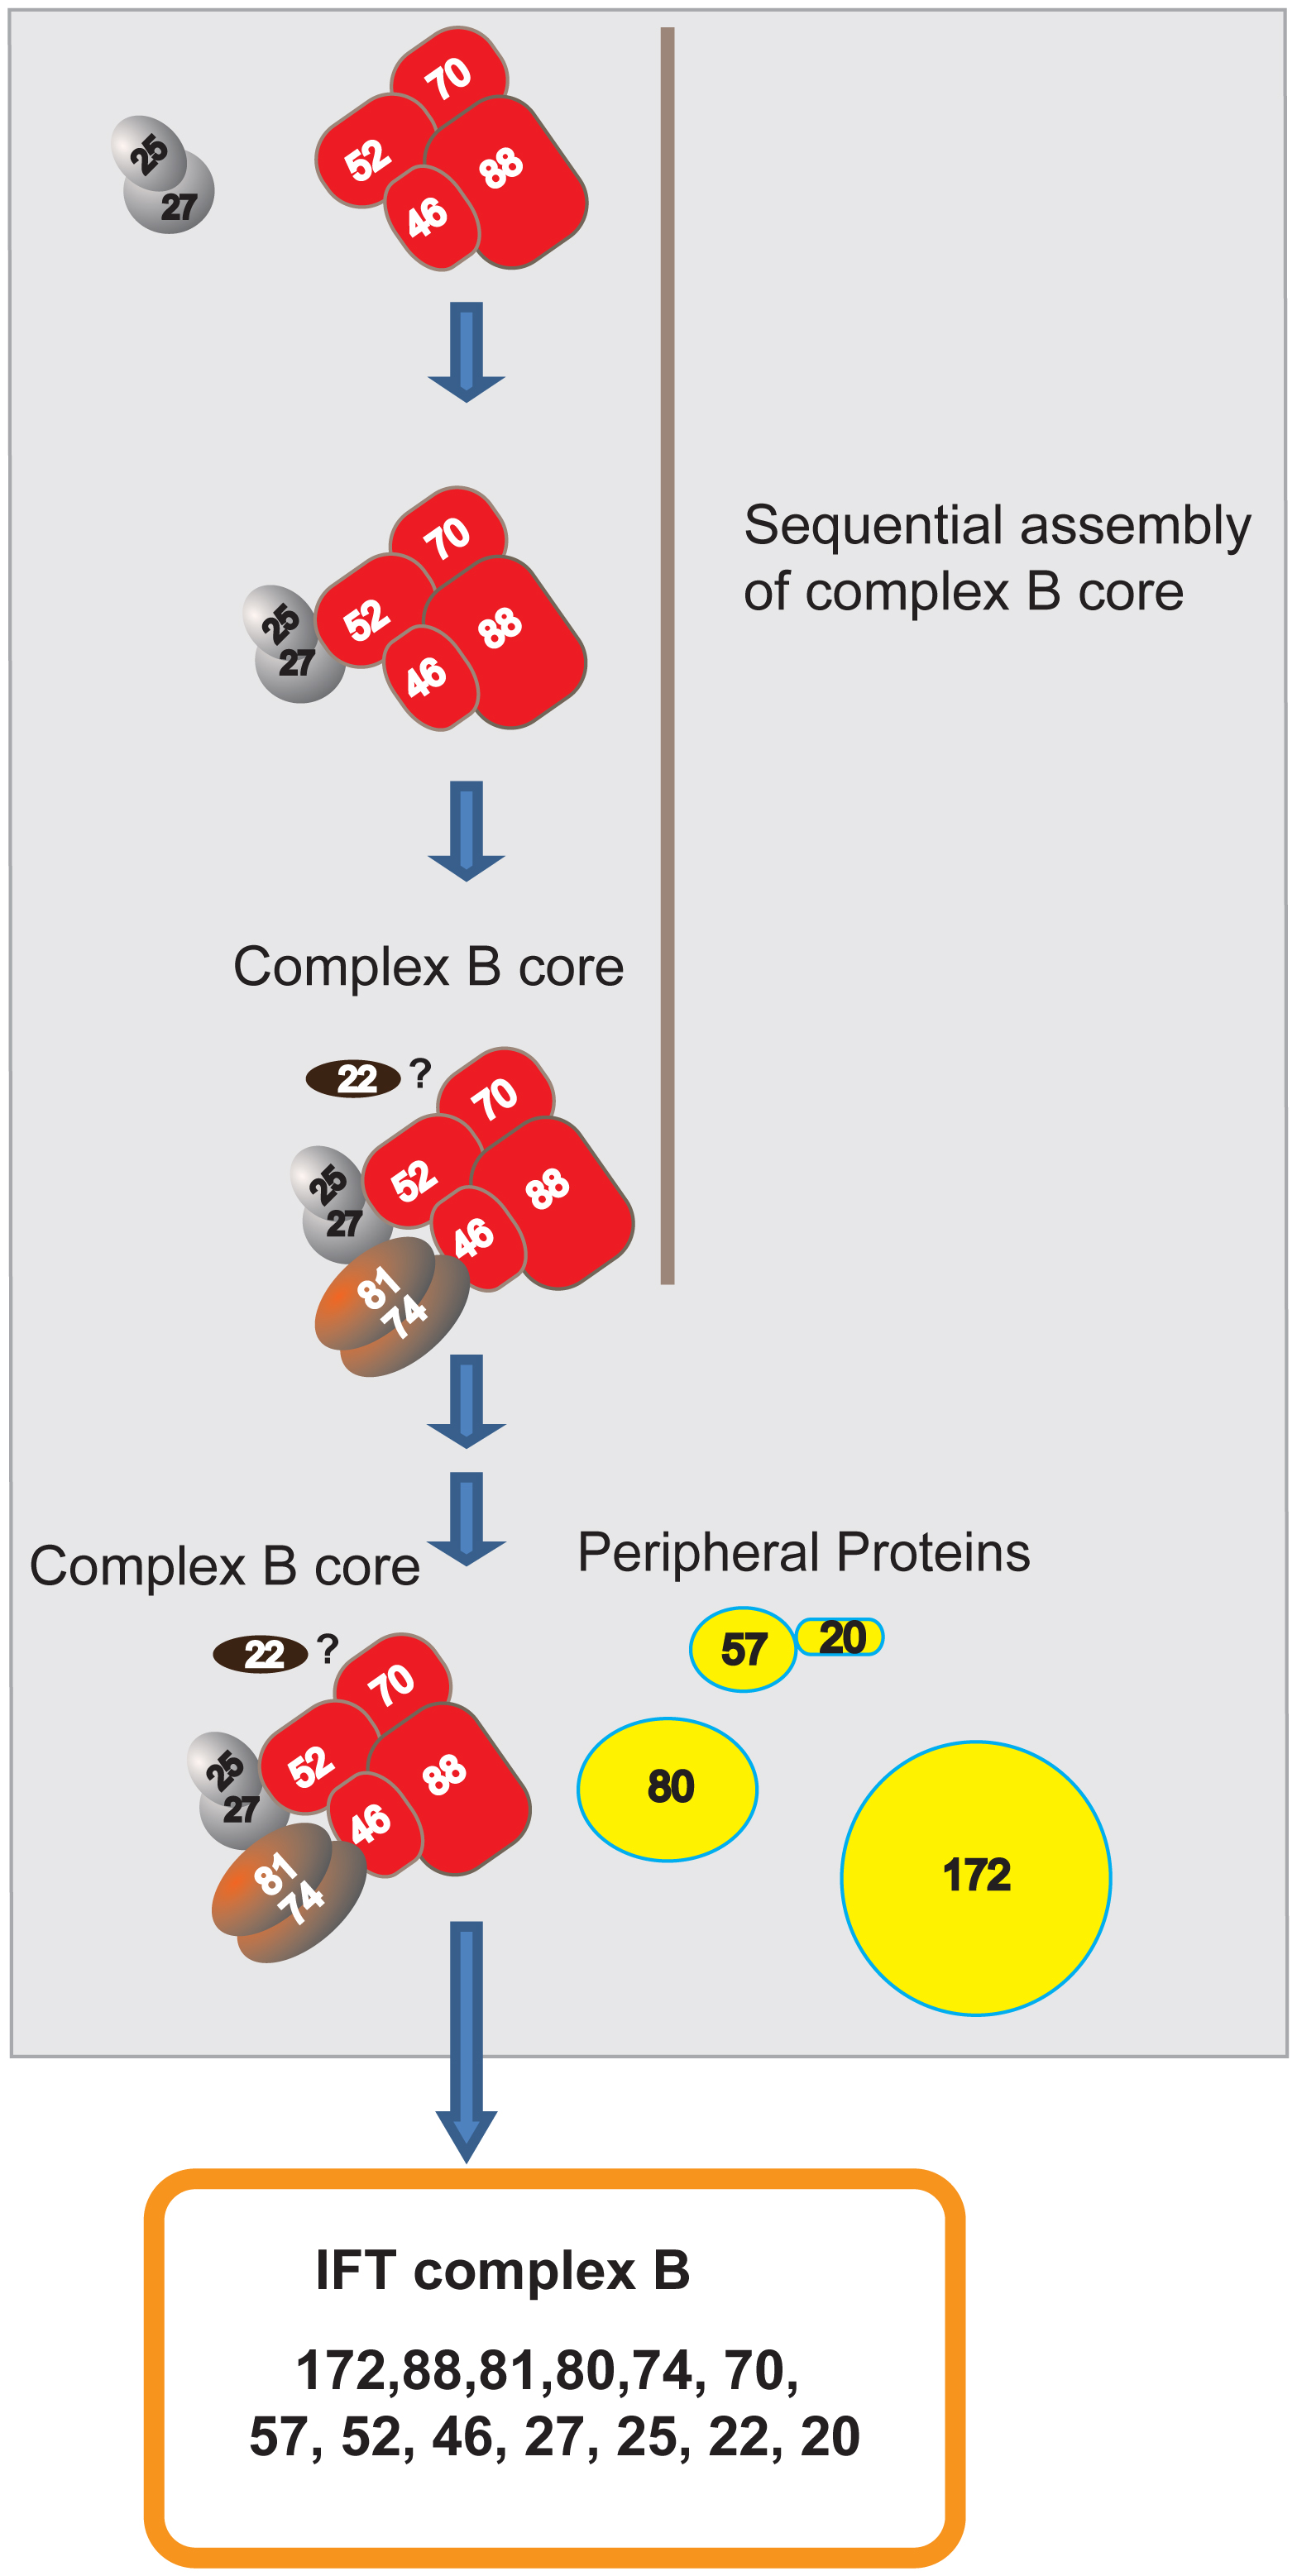
\includegraphics[width=\textwidth-85mm]{fig2-15.jpg}
%生成中英双语标题
{\setstretch{1.667}
\bicaption[fig:2.15]{图}{IFT-B的层级组装和基体定位模型\ \citep{Richey2012}。首先,
亚复合物\ IFT88/70/52/46\ 和\ IFT27/25\ 结合形成\ IFT88/70/52/46/27/25。该过程依赖\ IFT52。随后,IFT81\ 和\ IFT74\ 结合\ IFT88/70/52/46/27/25\ 形成\ IFT88/70/52/46/27/25/81/74。此步骤需要\ IFT46\ 的参与。最后,外周亚基组装到核心复合物上形成完整的复合物\ B。IFT88\ 对核心复合物的形成是非必须的,但它介导了外周亚基与核心复合物之间的结合。核心复合物的组装发生在基体远端,从远端转位到
过渡纤维依赖\ IFT88\ 及外周亚基的正常结合。} {Figure}{Sequential assembly and basal body localization of complex B \citep{Richey2012}. First, the subcomplexes IFT88/70/52/46 and IFT27/25 binds to form IFT88/70/52/46/27/25, and the binding is dependent on IFT52. Second, IFT74 and IFT81 assemble onto IFT88/70/52/46/27/25 to form IFT88/70/52/46/27/25/81/74. This step is assisted by IFT46. Lastly, the peripheral proteins assemble onto the complex B core to form an intact complex B. IFT88 is essential for mediating the binding of peripheral proteins to the B core. All the assembly steps involved in forming complex B core may occur at the proximal end of the basal bodies. The translocation from the proximal end of the basal body to the transition fibers dependents on the presence of IFT88 and proper association of peripheral proteins.}
\par}
%结束图片浮动体环境
\end{figure}

基于对\ IFT\ 复合物各亚基生化、遗传、定位和相互作用等方面的研究,\citet{Lucker2010}\ 提出了\ IFT\ 复合物\ B\ 的层级组装模型(图\ \ref{fig:2.14})。在该模型中,IFT88、IFT52\ 和\ IFT46\ 形成异源三聚体,IFT81\ 和\ IFT74/72\ 形成异源四聚体,IFT27\ 和\ IFT25\ 形成异源二聚体。这三个独立的亚复合物与其他亚基相互作用形成\ IFT\ 复合物\ B\ 的核心复合物。外周亚基随后与该核心相互作用形成完整的\ IFT\ 复合物\ B\ \citep{Lucker2010}。随
后,\citet{Richey2012}\ 基于对相关突变体进行的分析也提出了类似的模型(图\ \ref{fig:2.15})。他们认为\ IFT88、IFT70、IFT52\ 和\ IFT46\ 形成异源四聚体。该异源四聚体随后结合\ IFT27/IFT25\ 和\ IFT81/IFT74。通过以上步骤形成的\ IFT-B\ 核心复合物随后结合外周亚基形成完整的\ IFT-B\ \citep{Richey2012}。这两个模型虽然能够解释部分\ IFT\ 基因突变体的表型差异,但相关证据不够充分,需要进一步验证和研究。
%开始图片浮动体环境,其中!表示取消严谨限制,h表示在此处插入,t表示在本页或下一页顶部插入
\begin{figure}[htb!]
%居中对齐
\centering
%设置图片搜索路径,每个路径用{}括起来
\graphicspath{{figures/}}
%插入图片并设置图片宽度为文本宽度减10mm
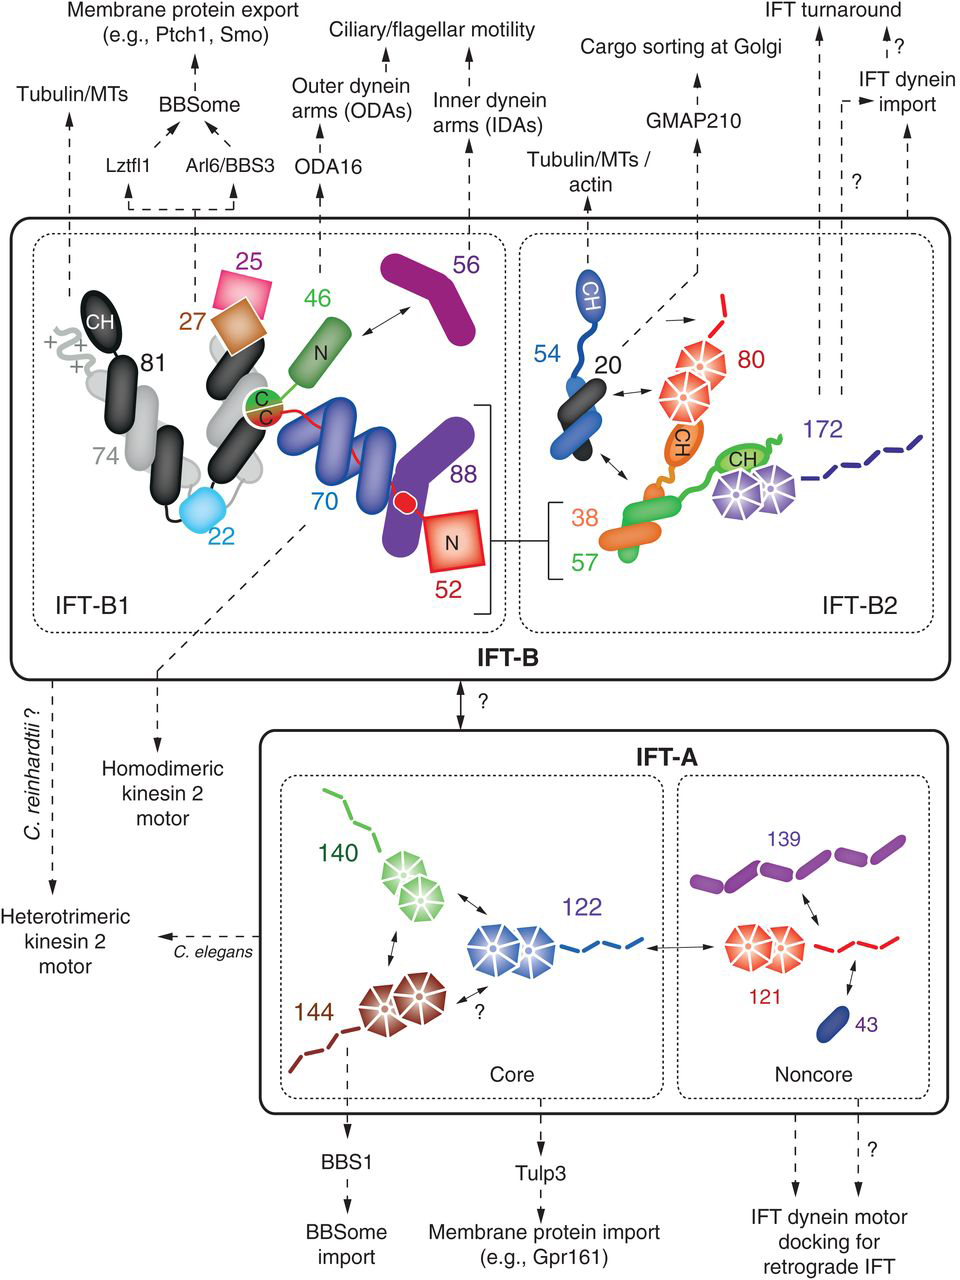
\includegraphics[width=\textwidth-30mm]{fig2-16.jpg}
%生成中英双语标题
{\setstretch{1.667}
\bicaption[fig:2.16]{图}{IFT\ 蛋白之间及\ IFT\ 蛋白与分子马达或货物之间的相互作
用\ \citep{Taschner2016}。MT\ 为微管,\textit{C. reinhardtii}\ 为莱茵衣藻,\textit{C. elegans}\ 为线虫。}{Figure}{Interactions within IFT proteins and interaction between IFT proteins/complexes and ciliary motor/cargo proteins \citep{Taschner2016}. MT, Microtubule; \textit{C. reinhardtii}, \textit{Chlamydomonas reinhardtii}; \textit{C. elegans}, \textit{Caenorhabditis elegans}.}
\par}
%结束图片浮动体环境
\end{figure}

近年来,Esben Lorentzen\ 教授率领的团队陆续解析了\ IFT-B\ 复合物中部分亚基及其货物的晶体结构\ (图\ \ref{fig:2.16}),如IFT25/27、IFT70/52、IFT52/46、IFT81/74/tubulin\ 和\ IFT46/ODA16 \citep{Bhogaraju2011,Taschner2014,Taschner2017,Bhogaraju2013a,Bhogaraju2014}。 同时他们还依据蛋白纯化结果将\ IFT-B\ 分为\ IFT-B1\ 和\ IFT-B2\ 两个子复合物\ (图\ \ref{fig:2.14})\citep{Taschner2016a}。这些研究虽然旨在解析\ IFT-B\ 及其与分子马达和货物的整体结构,但鉴于其与已知体内实验结果的高度吻合\ \citep{Kubo2016,Craft2015,Ahmed2008}。我们认为\ IFT\ 复合物的晶体结构可在一定程度上指导对\ IFT\ 蛋白基体定位的相关研究。然而,体内实验长期以来受到有限的突变体和抗体的制约。此外,研究多亚基复合物组装的方法和手段也很匮乏。

相比于\ IFT-B\ 复合物中的亚基,对\ IFT-A\ 复合物中亚基的基体定位相关研究较少。原因之一是\ IFT-A\ 中的亚基分子量普遍较大。\citet{Brown2015}\ 发现\ IFT-A\ 和\ IFT-B\ 在野生型衣藻的基体共定位。然而,这种共定位在\ \textit{IFT74}\ 的缺失突变体\ \textit{ift74-2}\ 中消失。这一结果表明\ IFT-A\ 和\ IFT-B\ 通过独立的方式定位到基体。在已有的研究中,IFT-A\ 在\ IFT-B\ 亚基的缺失突变体中能够正常定位到基体。反之,IFT-B\ 在\ IFT-A\ 亚基的缺失突变体中也能够正常定位到基体\ \citep{Behal2012,Brown2015,Hou2007,Richey2012}。此外,前面提到的\ CPLANE\ 蛋白能够招募\ IFT-A\ 外周亚基,而非\ IFT-A\ 核心亚基或\ IFT-B\ 定位到基体\ \citep{Toriyama2016}。 这些结果进一步验证了“预组装-定位”模型。

在未来的研究中,我们需要确定到底哪些亚基和货物在定位到基体之前已经预组装成亚
复合物\ \citep{Lechtreck2015,Lechtreck2017,Taschner2016,Fu2016}。同时我们还需要探究这些亚复合物的组装次序。这些研究有助于最终阐明\ IFT\ 蛋白基体定位以及与货物相互作用的机制。这对解析纤毛的组装与解聚机理至关重要。同时,这些研究对调控纤毛形成及纤毛功能和纤毛病的预防与治疗也具有重要的指导意义。